\documentclass[11pt]{article}
\usepackage[T1]{fontenc}
\usepackage[utf8]{inputenc}
\usepackage{lmodern}
\usepackage[margin=1.05in]{geometry}
\usepackage{amsmath,amssymb,amsthm,mathtools}
\usepackage{enumitem,booktabs,microtype}
\usepackage{tikz}
\usetikzlibrary{arrows.meta,positioning,calc}
\usepackage[numbers,sort&compress]{natbib}
\usepackage{xurl}
\usepackage[colorlinks=true,linkcolor=blue,citecolor=blue,urlcolor=blue,
  pdftitle={Finite algebraic envelopes and the Boone--Higman conjecture},
  pdfauthor={OpenAI}]{hyperref}
\newtheorem{theorem}{Theorem}[section]
\newtheorem{lemma}[theorem]{Lemma}
\newtheorem{proposition}[theorem]{Proposition}
\newtheorem{corollary}[theorem]{Corollary}
\theoremstyle{definition}
\newtheorem{definition}[theorem]{Definition}
\theoremstyle{remark}
\newtheorem{remark}[theorem]{Remark}
\newcommand{\F}{\mathbb F}
\newcommand{\St}{\operatorname{St}}
\newcommand{\E}{\operatorname{E}}
\newcommand{\eps}{\varepsilon}
\newcommand{\op}{\mathrm{op}}
\DeclareMathOperator{\im}{im}
\DeclareMathOperator{\diag}{diag}
\setlist[enumerate]{itemsep=3pt,topsep=5pt}
\setlist[itemize]{itemsep=3pt,topsep=5pt}
\setlength{\emergencystretch}{1.5em}
\title{Finite algebraic envelopes and the Boone--Higman conjecture}
\author{OpenAI}
\date{September 23, 2026}
\begin{document}
\maketitle
\begin{abstract}
We prove the Boone--Higman conjecture. A finitely generated group has
decidable word problem if and only if it embeds in a finitely presented
simple group.
\end{abstract}
\tableofcontents
\section{Introduction}\label{sec:introduction}

The word problem for a group with a specified finite generating set asks
whether a given word in the generators and their inverses represents the
identity. It is \emph{decidable} if an algorithm answers this question for
every word. A group is \emph{simple} here if it is nontrivial and its only
normal subgroups are the identity subgroup and the whole group.

\begin{theorem}\label{thm:main}
For every finitely generated group \(G\), the following are equivalent:
\begin{enumerate}[label=\textup{(\roman*)}]
\item \(G\) has decidable word problem.
\item \(G\) embeds in a finitely presented simple group.
\end{enumerate}
\end{theorem}

An embedding throughout means an injective group homomorphism. In the
constructive implication, \(G\) is supplied with a finite generating set
and a word-problem decider; it need not be finitely presented.
Theorem~\ref{thm:main} resolves the Boone--Higman conjecture positively.

Higman's embedding theorem characterizes the finitely generated
subgroups of finitely presented groups as those admitting a recursively
enumerable set of defining relations \cite{Higman61}; see also
\cite[Theorem~A]{AanderaaCohen1980}.
Decidability of the word problem is stronger: it supplies an algorithm
for both equality and inequality. Boone and Higman characterized this
condition by the existence of embeddings
\[
 G\ \leq\ H\ \leq\ K,
 \qquad H\text{ simple},\quad K\text{ finitely presented}
\]
\cite[Theorem~I]{BH74}. They asked whether the simple overgroup \(H\)
could itself be chosen finitely presented \cite[p.~43]{BH74}.
The two properties in their theorem belong to different groups, and
finite presentation does not in general pass to subgroups.
Thompson subsequently obtained a finitely generated simple overgroup
with decidable word problem \cite{Tho80}; a later proof appears in
\cite[Theorem~7.1]{DarbinyanSteenbock2022}.
This strengthens the conclusion to finite generation of the simple
overgroup, but does not supply its finite presentation.

Positive cases of the conjecture include hyperbolic and contracting
self-similar groups \cite[Theorem~A and Corollary~D]{BBMZhyperbolic},
Baumslag--Solitar groups and finite-rank free-by-cyclic groups
\cite[Theorem~A]{BuxLlosaWu2025}, and automorphism groups of finite-rank
free groups and mapping class groups of orientable punctured surfaces
of finite type \cite[Theorem~A and Corollary~B]{BFFHZ}.
The survey \cite{BBMZsurvey} describes further results and the
development of the conjecture.

Our principal intermediate result concerns permutation actions.
An action on a set \(X\) is \emph{faithful} if only the identity acts
trivially, and \emph{two-transitive} if it is transitive on the ordered
pairs of distinct points of \(X\).

\begin{theorem}\label{thm:envelope}
Every finitely generated group with decidable word problem embeds in a
finitely presented group \(\Gamma\) admitting a faithful two-transitive
action on a countably infinite set. Every point stabilizer of this action
is finitely generated.
\end{theorem}

The action is designed for the twisted Brin--Thompson construction of
Belk and Zaremsky, which embeds an acting group in a simple group
\cite[Section~3 and Theorem~3.4]{BelkZaremsky2022}.
Their original finite-presentation theorem used finitely many orbits on
finite subsets of each size and finitely presented finite-set
stabilizers \cite[Theorem~D]{BelkZaremsky2022}.
Zaremsky subsequently showed that finite presentation of the acting
group, finite generation of point stabilizers, and finitely many orbits
on unordered pairs suffice
\cite[Theorem~A and Corollary~B]{Zaremsky2024Finite}.
Two-transitivity supplies the last condition here. We state this
criterion precisely in Theorem~\ref{thm:zaremsky}; the construction below
provides its faithful action and the embedding of the prescribed group.

\subsection*{The proof}

The action is affine. Translations move the first point of an ordered
pair to zero, so two-transitivity reduces to transitivity of the linear
part on nonzero vectors. A simple algebra \(A\) provides the required
coefficient operations: if \(0\ne m\in A\), then its identity belongs
to \(AmA\), and hence is a finite sum of left and right multiples of
\(m\). Elementary row operations can use this identity to move vectors.
Finite presentation, however, will come from a different algebra.

Over \(k=\F_2\), we construct a finitely presented algebra \(B\), a
simple subalgebra \(A\subseteq B\) with its own identity, and an
injective nonunital map \(\phi:B\to B\) with image in \(A\).
The additive direct limit \(M_\infty=\varinjlim(B,\phi)\) is the
carrier for the action on \(X=M_\infty^6\). Every finite collection
of its coordinates lies in one copy of \(B\); advancing once places
them in \(A\). Thus simplicity becomes available at a later stage
without requiring the finitely presented algebra \(B\) itself to be
simple.

The coefficient ring \(R=B\otimes_k B^{\op}\) acts on \(B\) by
left and right multiplication. We give an explicit finite presentation
of the affine Steinberg group
\[
 \Gamma_0=B^6\rtimes\St_6(R).
\]
The Steinberg group maps onto the elementary matrix group \(\E_6(R)\),
but its kernel is an obstruction to the desired faithful affine action.
We remove that entire kernel by a single application of the coefficient
map induced by \(\phi\). The key algebraic input consists of two
splitting pairs commuting with the coefficient image. Their corner
identities give an exact calculation in the Steinberg presentation;
no centrality hypothesis on the kernel is needed.

The resulting endomorphism of \(\Gamma_0\) defines a finitely
presented mapping torus \(\Gamma\). In its direct-limit description
the Steinberg kernel has disappeared, leaving elementary matrices acting
on \(M_\infty^6\), together with translations and a stage shift.
Simplicity of \(A\) gives the nonzero-vector orbit required for
two-transitivity. Faithfulness uses two further properties of the
algebra construction: a separating vector detects every nonzero
coefficient after one advance, and the proper support
\(\phi(1_B)\ne1_B\) makes the stage shift detectable. The stabilizer
of zero is the quotient by the translation subgroup, so it is finitely
generated. To embed the original \(G\), we first use an HNN extension
to express its elements as controlled commutators; balanced elementary
diagonals then place this copy of \(G\) in the linear part.

It remains to construct the algebras with these simultaneous properties.
We do so through a finitely presented monoid and a decidable monoid that
encode one another. A finite presentation is compiled syntactically from
a program index, before any totality assertion is available. Its partial
evaluator controls the length of every call to the encoded program.
Long codes make the calls needed to normalize a word strictly shorter
than that word. A fixed-point argument and induction on length then
establish totality and compatibility with multiplication.
Finite-tuple selectors isolate individual basis terms in a contracted
monoid algebra, producing \(A\); a separate separator distinguishes
ordered pairs of basis terms, producing the faithful coefficient detector.

The finite-presentation construction follows the machine-encoding
tradition of Post and Murskii \cite{Post1947,Murskii1967}.
Here the bounded evaluator permits the two monoids to be constructed
together. The selectors strengthen the contextual-collapse property in
the semigroup counterpart of the Boone--Higman theorem
\cite[pp.~49--52]{BH74}: isolating each term of a finite linear
combination gives the simplicity needed for the affine action.

Section~\ref{sec:reduction} states the algebraic data and gives the
HNN reduction.
Sections~\ref{sec:affine}--\ref{sec:action} construct the action and prove
the two theorems from those data.
Section~\ref{sec:algebra} constructs the algebras from a precise monoid
theorem, proved by bounded self-reference in Section~\ref{sec:bootstrap}.
Appendix~\ref{sec:compiler} gives the full finite compiler and its
evaluator proof.

\section{The group input and the algebraic data}\label{sec:reduction}

We first enlarge the input group so that each of its elements is a
commutator in the larger group. This will allow us to embed the input
group in an elementary matrix group in Section~\ref{sec:action}.
We then state the algebraic construction used in the next three
sections. All rings and algebras have identities; a homomorphism
explicitly called nonunital is not required to preserve them.
Our commutator convention is \([a,b]=aba^{-1}b^{-1}\).

\begin{lemma}\label{lem:group-input}
Let \(G\) be finitely generated with decidable word problem. There is a
finitely generated group \(\widehat G\) with decidable word problem
containing \(G\times G\), and an element \(s\in\widehat G\), such that
\[
 [(g,g),s]=(g,1)\qquad(g\in G).
\]
\end{lemma}
\begin{proof}
Take the HNN extension
\[
 \widehat G=
 \left\langle G\times G,s\ \middle|\
 s(g,g)s^{-1}=(1,g)\quad(g\in G)\right\rangle .
\]
The associated subgroups are the diagonal and the second factor, with
the indicated isomorphism. Britton's Lemma embeds the base
\cite{Britton63}; see also the precise effective HNN formulation in
\cite[p.~44]{BH74}.

We spell out the decision procedure. Store each base word as a pair of
words on the given generators of \(G\). Membership of \((a,b)\) in the
diagonal is decided by testing \(ab^{-1}=1\), and membership in the second
factor by testing \(a=1\). Replace each available pinch by
\[
 s(a,a)s^{-1}\longmapsto(1,a),
 \qquad
 s^{-1}(1,b)s\longmapsto(b,b),
\]
and multiply adjacent base words. Each pinch removes two stable letters.
When no pinch remains, a word still containing a stable letter is
nontrivial by Britton's Lemma. Otherwise decide the resulting base word
coordinatewise. Thus the procedure terminates and decides the word
problem, without requiring a finite presentation of \(G\).
The two copies of a finite generating set, together with \(s\), generate
\(\widehat G\). Finally,
\[
 [(g,g),s]=(g,g)\,s(g^{-1},g^{-1})s^{-1}
           =(g,g)(1,g^{-1})=(g,1).
\]
This includes finite groups and the trivial group; in the latter case
\(\widehat G\) is infinite cyclic.
\end{proof}

Here is the algebraic construction. A simple algebra means a nonzero
algebra with no proper nonzero two-sided ideal. A subalgebra with identity
\(e\) need not contain the identity of the ambient algebra; its units
are taken relative to \(e\). For an idempotent \(q\in B\), the
subalgebra \(qBq=\{qbq:b\in B\}\) is called a \emph{corner};
its identity is \(q\).

\begin{theorem}\label{thm:algebra-package}
For every finitely generated group \(L\) with decidable word problem,
there are the following data over \(k=\F_2\):
\begin{enumerate}[label=\textup{(\roman*)}]
\item A nonzero finitely presented unital algebra \(B\), a simple
subalgebra \(A\subseteq B\) with identity \(e\), and an embedding
\(L\hookrightarrow A^\times\).
\item An injective nonunital algebra homomorphism \(\phi:B\to B\) with
\(\phi(B)\subseteq A\) and \({p=\phi(1_B)\ne1_B}\).
\item Elements \(s_0,s_1,t_0,t_1\in pBp\) commuting with \(\phi(B)\)
and satisfying
\[
 t_i s_j=\delta_{ij}p,\qquad s_0t_0+s_1t_1=p
 \quad(i,j\in\{0,1\}).
\]
\item An element \(b_*\in B\) with the following property. Put
\[
 R=B\otimes_k B^{\op},\qquad
 \psi=\phi\otimes\phi^{\op},
 \qquad (a\otimes b^{\op})\cdot m=amb.
\]
Then
\[
 r\ne0\ \Longrightarrow\ \psi(r)\cdot b_*\ne0
 \qquad(r\in R).
\]
\end{enumerate}
\end{theorem}

Theorem~\ref{thm:algebra-package} is proved in
Section~\ref{sec:algebra}, using the monoid construction of
Section~\ref{sec:bootstrap} and Appendix~\ref{sec:compiler}.
To see how these data produce an action, regard the elements of \(R\)
as coefficients for row operations on \(B^6\). Such a coefficient
acts on a coordinate by a finite sum of left and right multiplications.
Simplicity of \(A\) will let a nonzero coordinate produce any prescribed
element of \(A\); applying \(\phi\) places all coordinates in that
subalgebra. Finite presentation of \(B\) supplies a finitely presented
Steinberg group acting by row operations. The splitting pairs make its matrix
kernel disappear under the induced coefficient map, while \(b_*\)
detects every remaining nonidentity matrix after that map is applied.
Finally, the support identity \(p\ne1_B\) makes successive vector
stages strictly larger, so that shifting stages gives a nontrivial
permutation. Sections~\ref{sec:affine}--\ref{sec:action} establish these
claims and assemble the action.

In particular, \(p\phi(b)=\phi(b)p=\phi(b)\), so
\(1_B\notin\phi(B)\). The detection condition concerns the action
after applying \(\psi\); it does not require the original action of
\(R\) on \(B\) to be faithful.

Apply the theorem with \(L=\widehat G\) from
Lemma~\ref{lem:group-input}. For the remainder of
Sections~\ref{sec:affine}--\ref{sec:action}, fix these data. Tensor
products are over \(k\). Besides \(p\), define
\[
 P=p\otimes p^{\op},\qquad
 U_i=s_i\otimes p^{\op},\qquad
 V_i=t_i\otimes p^{\op}.
\]
Tensoring injective linear maps over a field shows that \(\psi\) is
injective, so \(P\ne0\). Also \(P\ne1_R\), since the nonzero tensor
\((1_B-p)\otimes1_B\) annihilates \(P\) on the left.
The elements \(U_i,V_i\) lie in \(PRP\), commute with
\(\psi(R)\), and satisfy
\begin{equation}\label{eq:ring-pairs}
 V_iU_j=\delta_{ij}P,\qquad U_0V_0+U_1V_1=P.
\end{equation}
These identities follow directly from the corresponding identities
in \(B\); the second tensor factor is always the idempotent \(p^{\op}\).

The final passage from an action to a simple group uses the following
established result, in the precise form needed here.

\begin{theorem}[Zaremsky]\label{thm:zaremsky}
Suppose a finitely presented group \(\Lambda\) acts faithfully on a
nonempty countable set \(X\). If the point stabilizers are finitely
generated and there are finitely many orbits on the unordered
two-element subsets of \(X\), then \(\Lambda\) embeds in a nontrivial
finitely presented simple group.
\end{theorem}

These are the hypotheses of a type-\textup{(A)} action in
\cite[Theorem~A and Corollary~B]{Zaremsky2024Finite}.
Finite presentation follows from that theorem; the canonical embedding
and simplicity are those of the twisted Brin--Thompson construction
\cite[Section~3 and Theorem~3.4]{BelkZaremsky2022}. Since \(X\) is nonempty, the
constructed group contains Thompson's group \(V\) on a coordinate and
is nontrivial. Our construction will provide a countably infinite \(X\)
with one orbit on pairs, and will prove each of the other hypotheses
separately.

\section{A finitely presented affine group}\label{sec:affine}

We now use the algebraic data in Theorem~\ref{thm:algebra-package} to
construct a finitely presented group of translations and elementary
operations.  The translations form the additive group of $B^6$.
We first give their finite presentation relative to a Steinberg group,
and then construct the endomorphism used in the next two sections.

\subsection{The coefficient ring and the translation module}

Put
\[
 R=B\otimes_k B^{\op},
 \qquad (a\otimes b^{\op})\cdot m=amb\quad(m\in B).
\]
Thus $r=\sum_\nu a_\nu\otimes b_\nu^{\op}$ acts on $B$ by the
operation $m\mapsto\sum_\nu a_\nu m b_\nu$. The opposite multiplication
in the second factor makes composition of these operations agree with
multiplication in $R$, so $B$ is a left $R$-module.
The ring $R$ is finitely presented
as a unital associative ring: take a finite algebra presentation of
$B$, a second copy with products reversed, the relations commuting
every generator of the first copy with every generator of the second,
and $2\cdot1=0$.  The universal property of the tensor product
identifies the resulting ring with $R$.
The module $B$ is generated by $1_B$; we next show that the relations
on this module generator also have a finite description.

\begin{lemma}\label{lem:cyclic-module}
Let $Y$ be a finite algebra generating set for $B$.  For $b\in B$ put
\[
 d_b=b\otimes1-1\otimes b^{\op},
 \qquad J=\sum_{y\in Y}R d_y.
\]
Evaluation at $1_B$ induces an isomorphism of left $R$-modules
$R/J\cong B$.
\end{lemma}

\begin{proof}
Evaluation is a surjective $R$-module homomorphism, and every $d_y$
annihilates $1_B$.  The identity
\begin{equation}\label{eq:module-product}
 d_{bc}=(b\otimes1)d_c+(1\otimes c^{\op})d_b
\end{equation}
shows, together with additivity and $d_1=0$, that $d_b\in J$ for all
$b\in B$.  Indeed, $B$ is generated by $Y$ over the prime field $k$.
Consequently
\[
 a\otimes b^{\op}\equiv ab\otimes1\pmod J
 \qquad(a,b\in B).
\]
Every element of $R$ is therefore congruent modulo $J$ to its
evaluation tensored with $1$.  The additive map
$b\mapsto(b\otimes1)+J$ is an inverse to the induced evaluation map.
Thus the kernel is exactly the stated left ideal.
\end{proof}

For a unital ring $R$ and $n\geq3$, the Steinberg group $\St_n(R)$
has generators $x_{ab}(r)$, where $1\leq a\ne b\leq n$ and $r\in R$,
with relations
\begin{align}
 x_{ab}(r)x_{ab}(s)&=x_{ab}(r+s),\label{eq:steinberg-add}\\
 [x_{ab}(r),x_{bc}(s)]&=x_{ac}(rs)
       &&(a,b,c\text{ distinct}),\label{eq:steinberg-product}\\
 [x_{ab}(r),x_{cd}(s)]&=1
       &&(a\ne d,\ b\ne c).\label{eq:steinberg-commute}
\end{align}
Let $e_{ab}$ denote the matrix unit.  The map
$x_{ab}(r)\mapsto I+r e_{ab}$ gives a surjection
\[
 \pi_n:\St_n(R)\longrightarrow\E_n(R),
\]
where $\E_n(R)$ is the subgroup of $\mathrm{GL}_n(R)$ generated by
these elementary matrices.  Krsti\'c and McCool prove that
$\St_n(R)$ is finitely presented whenever $R$ is a finitely presented
unital associative ring and $n\geq4$
\cite[Theorem~3]{KrsticMcCool1999}.  Their theorem permits
noncommutative rings, and applies to the ring constructed above.

\subsection{A finite relative presentation}

The next lemma supplies the additional relations needed for the
translations.  Finite presentation of the module and of the linear
group alone would not establish its conclusion; we prove the
semidirect-product presentation explicitly.

\begin{lemma}\label{lem:affine-presentation}
Let $R$ be a finitely generated unital associative ring, let
$J=\sum_{d\in D}Rd$ for a finite subset $D\subset R$, and let $n\geq4$.
If $\St_n(R)$ is finitely presented, then
\[
 (R/J)^n\rtimes\St_n(R)
\]
is finitely presented, where the action on columns is induced by
$\pi_n$.  More precisely, choose a finite ring generating set
$F\subset R$ containing $1$.  A finite presentation is obtained
from a finite presentation of $\St_n(R)$ by adjoining
$p_1,\ldots,p_n$ and the relations
\begin{align}
 [p_a,p_b]&=1,\label{eq:affine-p}\\
 [x_{ab}(s),p_c]&=1
     &&(s\in F,\ c\ne b),\label{eq:affine-central}\\
 [x_{ab}(1),p_b]&=p_a,\label{eq:affine-unit}\\
 [x_{ab}(d),p_b]&=1
     &&(d\in D).\label{eq:affine-ideal}
\end{align}
Here every root has $a\ne b$, and each root occurring in these
finitely many relations is represented by a word in the chosen
generators of $\St_n(R)$.
\end{lemma}

\begin{proof}
Let $Q$ be the group given by this presentation. In the intended
semidirect product, $p_a$ translates by $1+J$ in row $a$, and
$[x_{ab}(r),p_b]$ translates by $r+J$ in that row. We recover these
translations and their elementary action from the finite relations,
working inside $Q$ until the final inverse-homomorphism argument.

\paragraph{Coefficients.}
Relation~\eqref{eq:affine-central} holds for every $s\in R$.
To see this, let $C$ be the set of coefficients for which it holds
for every permitted triple of indices.  By
\eqref{eq:steinberg-add}, $C$ is an additive subgroup containing
$F$.  If $r,s\in C$, choose $h\notin\{a,b,c\}$.  There is such an
index because $n\geq4$.  Then
\[
 x_{ab}(rs)=[x_{ah}(r),x_{hb}(s)],
\]
and both factors commute with $p_c$.  Thus $C$ is closed under
multiplication, so $C=R$.

\paragraph{Independence of a column.}
For $a\ne b$, define
\[
 w_a^b(r)=[x_{ab}(r),p_b].
\]
If $h$ differs from $a,b$, then $w_a^b(r)$ commutes with $p_h$:
both $x_{ab}(r)$ and $p_b$ do.  Put
\[
 X=x_{ah}(r),\qquad Y=x_{hb}(1),\qquad Z=x_{ab}(r).
\]
The Steinberg relation $[X,Y]=Z$ gives $XY=ZYX$.
Conjugating $p_b$ by these equal products yields
\begin{align*}
 (XY)p_b(XY)^{-1}&=w_a^h(r)p_hp_b,\\
 (ZYX)p_b(ZYX)^{-1}&=p_hw_a^b(r)p_b.
\end{align*}
Here $X$ fixes $p_b$, $Y$ sends $p_b$ to $p_hp_b$, and $Z$ fixes
$p_h$.  Cancelling $p_b$ and using the preceding commutation with
$p_h$ proves $w_a^h(r)=w_a^b(r)$.  We write this common value as
$w_a(r)$.

\paragraph{Commutations.}
The element $w_a(r)$ commutes with every $p_c$: choose its defining
column $b\notin\{a,c\}$, so that both defining factors commute with
$p_c$.  It also commutes with $x_{cd}(s)$ whenever $d\ne a$.
For this, choose the defining column $b\notin\{a,c,d\}$.
Then $x_{ab}(r)$ commutes with $x_{cd}(s)$ by
\eqref{eq:steinberg-commute}, and $p_b$ commutes with $x_{cd}(s)$
because $b\ne d$.

These facts imply that all the $w$'s commute.  Given $w_a(r)$ and
$w_c(s)$, choose $b\notin\{a,c\}$ and write
$w_c(s)=[x_{cb}(s),p_b]$.  The element $w_a(r)$ commutes with both
factors, hence with their commutator.  This argument includes $a=c$.

\paragraph{Additivity.}
Using $[uv,p]=u[v,p]u^{-1}[u,p]$ and any $b\ne a$, we obtain
\begin{align*}
 w_a(r+s)
  &=[x_{ab}(r)x_{ab}(s),p_b]\\
  &=x_{ab}(r)w_a(s)x_{ab}(r)^{-1}w_a(r)\\
  &=w_a(r)w_a(s).
\end{align*}
The last equality uses the commutations just proved.  Thus
$w_a:(R,+)\to Q$ is a homomorphism.  Moreover,
$w_a(1)=p_a$ by \eqref{eq:affine-unit}.  In particular, any additive
torsion of $R$ is already imposed on these translations; in
characteristic two, $p_a^2=w_a(1+1)=1$.

\paragraph{Conjugation.}
It remains to determine the action of roots whose column is $a$.
For $c\ne a$, choose $b\notin\{a,c\}$ and put
\[
 X=x_{ca}(s),\qquad Y=x_{ab}(r),\qquad Z=x_{cb}(sr).
\]
The element $X$ fixes $p_b$, and $XYX^{-1}=ZY$.
Consequently
\begin{align}
 Xw_a(r)X^{-1}
    &=[ZY,p_b]
      =Zw_a(r)Z^{-1}w_c(sr)
      =w_a(r)w_c(sr).\label{eq:affine-action}
\end{align}
The last equality holds because the column $b$ of $Z$ differs
from $a$.  Together with the commutations already proved,
\eqref{eq:affine-action} is precisely the elementary action on
an additive column over the left module $R$.

\paragraph{The module relations.}
Relation~\eqref{eq:affine-ideal} says $w_a(d)=1$ for every $a$ and
$d\in D$.  To kill a left multiple in a prescribed row $c$, choose
$a\ne c$ and conjugate $w_a(d)=1$ by $x_{ca}(s)$.
Equation~\eqref{eq:affine-action} gives $w_c(sd)=1$.
Additivity now proves that every $w_c$ vanishes on $J$.

\paragraph{Inverse homomorphisms.}
Let $P_0=(R/J)^n\rtimes\St_n(R)$.  Sending $p_a$ to translation by
$1+J$ in row $a$ and using the identity on $\St_n(R)$ satisfies
all the defining relations of $Q$, and hence gives a homomorphism
$f:Q\to P_0$.  Conversely, the commuting additive maps
\[
 r+J\longmapsto w_a(r)
\]
define a homomorphism $(R/J)^n\to Q$.
Equation~\eqref{eq:affine-action} and the root commutations give
the required equivariance, so this map and the canonical map
$\St_n(R)\to Q$ induce $g:P_0\to Q$.
The composite $gf$ fixes $\St_n(R)$ and each
$p_a=w_a(1)$, so it is the identity on $Q$.
The composite $fg$ fixes $\St_n(R)$ and every translation:
in $P_0$, the commutator of $x_{ab}(r)$ with translation by $1+J$
in row $b$ is translation by $r+J$ in row $a$.
Thus $f$ and $g$ are inverse isomorphisms.
\end{proof}

\begin{proposition}\label{prop:affine}
For the algebra $B$ in Theorem~\ref{thm:algebra-package}, the group
\[
 \Gamma_0=B^6\rtimes\St_6(R),\qquad R=B\otimes_kB^{\op},
\]
is finitely presented.
\end{proposition}

\begin{proof}
The ring $R$ is finitely presented, so the Krsti\'c--McCool theorem
applies to $\St_6(R)$.  Lemma~\ref{lem:cyclic-module} identifies $B$
with a quotient of $R$ by a finitely generated left ideal.
Lemma~\ref{lem:affine-presentation}, with $n=6$, gives the result.
\end{proof}

\subsection{The transition endomorphism}

Write $\St=\St_6(R)$, $\E=\E_6(R)$, and
$\pi=\pi_6:\St\to\E$.  Recall the injective algebra map
$\phi:B\to B$ from Theorem~\ref{thm:algebra-package}, and set
$\psi=\phi\otimes\phi^{\op}:R\to R$.
This map is injective because tensoring vector spaces over $k$
preserves injections.  Both maps may be nonunital.

\begin{lemma}\label{lem:transition}
The formulas
\[
 \theta(x_{ab}(r))=x_{ab}(\psi(r)),\qquad
 \Theta(m,h)=(\phi^{(6)}(m),\theta(h))
\]
define endomorphisms of $\St$ and $\Gamma_0$, respectively.
Here $\phi^{(6)}$ acts componentwise on $B^6$.
The induced map on elementary matrices is the injective
homomorphism
\begin{equation}\label{eq:matrix-transition}
 F:\E\longrightarrow\E,
 \qquad F(g)=I+\psi^{(6)}(g-I),
\end{equation}
where $\psi^{(6)}$ means entrywise application on $6\times6$
matrices.  Thus $\pi\theta=F\pi$.
\end{lemma}

\begin{proof}
Additivity and multiplicativity of $\psi$ preserve all the
Steinberg relations, proving that $\theta$ is a homomorphism.
For an elementary tensor $r=a\otimes b^{\op}$ and $m\in B$,
\[
 \phi(r\cdot m)=\phi(amb)
   =\phi(a)\phi(m)\phi(b)
   =\psi(r)\cdot\phi(m).
\]
By additivity this holds for every $r\in R$.  Consequently, for
each elementary root,
\[
 \phi^{(6)}\bigl((I+r e_{ab})m\bigr)
   =(I+\psi(r)e_{ab})\phi^{(6)}(m).
\]
The roots generate $\St$, so this equivariance proves that
$\Theta$ is an endomorphism of the semidirect product.

For the matrix assertion, write $g=I+A$ and $h=I+C$.
Entrywise application of $\psi$ is additive and multiplicative
on matrix rings, even though it does not preserve their identity.
Since $gh-I=A+C+AC$, we have
\begin{align*}
 F(gh)
  &=I+\psi^{(6)}(A)+\psi^{(6)}(C)
       +\psi^{(6)}(A)\psi^{(6)}(C)\\
  &=F(g)F(h).
\end{align*}
Also $F(I)=I$, and the same calculation shows
$F(g^{-1})=F(g)^{-1}$.  On elementary matrices,
$F(I+r e_{ab})=I+\psi(r)e_{ab}$, proving both that $F$ maps
$\E$ into $\E$ and that $\pi\theta=F\pi$.
Finally, $F(g)=I$ forces every entry of $g-I$ to vanish because
$\psi$ is injective.  Thus $F$ is injective.
\end{proof}

We have obtained a finite presentation and compatible transition
maps.  The map $\Theta$ need not be injective: the remaining
obstruction lies in the kernel of $\pi$.  The next section proves
that $\theta$ annihilates this entire kernel.

\section{Annihilating the Steinberg kernel}\label{sec:kernel}

The affine group of Section~\ref{sec:affine} uses a Steinberg group,
whose matrix action can have a kernel.  We now show that the coefficient
endomorphism annihilates this entire kernel. The argument uses the
splitting pairs from Theorem~\ref{thm:algebra-package}, whose elements
commute with the coefficient image.
It is convenient to state it for an arbitrary unital associative ring.

Recall that $\operatorname{St}_6(R)$ has generators $x_{ij}(a)$, where
$1\leq i\ne j\leq6$ and $a\in R$, with relations
\begin{align}
 x_{ij}(a)x_{ij}(b)&=x_{ij}(a+b),\label{eq:kernel-additive}\\
 [x_{ij}(a),x_{jk}(b)]&=x_{ik}(ab)
       &&(i,j,k\text{ distinct}),\label{eq:kernel-chain}\\
 [x_{ij}(a),x_{kl}(b)]&=1
       &&(i\ne l,\ j\ne k).\label{eq:kernel-distant}
\end{align}
Here $[u,v]=uvu^{-1}v^{-1}$.  Let
$\pi:\operatorname{St}_6(R)\to\operatorname{E}_6(R)$ send
$x_{ij}(a)$ to $I+ae_{ij}$.

\begin{theorem}\label{thm:kernel}
Let $R$ be a unital associative ring, let $\psi:R\to R$ be an additive
multiplicative map, and put $P=\psi(1)$.  Suppose that
$U_0,U_1,V_0,V_1\in PRP$ commute with $\psi(R)$ and satisfy
\[
 V_iU_j=\delta_{ij}P,\qquad U_0V_0+U_1V_1=P.
\]
Then the homomorphism
\[
 \theta:\operatorname{St}_6(R)\longrightarrow\operatorname{St}_6(R),
 \qquad x_{ij}(a)\longmapsto x_{ij}(\psi(a)),
\]
satisfies $\theta(\ker\pi)=1$.
\end{theorem}

For the binary Leavitt algebra $L=L_{\F_2}(1,2)$, Khanh proves that
the natural map $\St_r(L)\to\mathrm{GL}_r(L)$ is an isomorphism for
$r\ge3$ \cite[Theorem~5.4]{Khanh2026Leavitt}.
Theorem~\ref{thm:kernel} concerns an arbitrary ring and annihilation
of its matrix kernel under the specified coefficient map.

Additivity and multiplicativity make $\theta$ a homomorphism by the
defining relations.  The map $\psi$ need not preserve the identity.
For any additive
multiplicative map $\lambda:R\to R$, the corresponding image of a root
word with matrix $g$ has matrix
\begin{equation}\label{eq:kernel-nonunital}
 I+\lambda^{(6)}(g-I),
\end{equation}
where $\lambda^{(6)}$ acts entrywise.  This follows on generators and
then on products by expanding $gh-I=(g-I)+(h-I)+(g-I)(h-I)$.
In particular, coefficient maps preserve the condition of having
identity matrix.  We shall use this for maps whose images lie in
smaller idempotent corners of $R$.

The proof has two parts.  First, a word with identity matrix becomes
central when all its coefficients are placed in a suitable corner.
Second, two orthogonal copies of that corner can be interchanged and
split.  Four corners suffice to make the resulting central element
equal to its square.

\subsection{Conjugation with an unused index}

The use of an index outside the support of a root word is the classical
Steinberg centrality argument; see
\cite[proof of Theorem~III.5.2.1]{Weibel2013}.
We record its row-and-column form to justify the corner conjugations
inside the Steinberg group. The kernel-annihilation theorem also uses
the corner comparisons and four-corner splitting proved below.

\begin{lemma}\label{lem:external-roots}
Let $J\subseteq\{1,\ldots,6\}$ and $k\notin J$.  For a column $c$ and
a row $r$ indexed by $J$, put
\[
 C_k(c)=\prod_{i\in J}x_{ik}(c_i),\qquad
 R_k(r)=\prod_{i\in J}x_{ki}(r_i).
\]
If $w$ is a root word using only indices in $J$, and $A$ is its matrix
on those indices, then
\begin{equation}\label{eq:external-action}
 wC_k(c)w^{-1}=C_k(Ac),\qquad
 wR_k(r)w^{-1}=R_k(rA^{-1}).
\end{equation}
Consequently, an element represented by a root word omitting index $6$
and having identity matrix is central in $\operatorname{St}_6(R)$.
\end{lemma}

\begin{proof}
The factors in each defining product commute.  It suffices to check
conjugation by $x_{ij}(a)$ with $i,j\in J$.  Its only changed column
factor and row factor are, respectively,
\begin{align*}
 x_{ij}(a)x_{jk}(c_j)x_{ij}(a)^{-1}
    &=x_{ik}(ac_j)x_{jk}(c_j),\\
 x_{ij}(a)x_{ki}(r_i)x_{ij}(a)^{-1}
    &=x_{kj}(-r_i a)x_{ki}(r_i).
\end{align*}
The first identity is \eqref{eq:kernel-chain}.  For the second,
reverse the relation
$[x_{ki}(r_i),x_{ij}(a)]=x_{kj}(r_i a)$.
These operations are multiplication of a column by $I+ae_{ij}$ and
of a row by $I-ae_{ij}$.  Composition proves
\eqref{eq:external-action} inside the Steinberg group.

If $w$ omits $6$ and has identity matrix, it therefore commutes with
every $x_{i6}(a)$ and $x_{6i}(a)$.  It commutes with every remaining
root as well, since
\[
 x_{ij}(a)=[x_{i6}(a),x_{6j}(1)]\qquad(i,j\ne6).
\]
These roots generate the group.
\end{proof}

\begin{lemma}\label{lem:corner-centrality}
Let $E,F\in R$ be idempotents with $EF=FE=0$.  Suppose $d,d^*\in R$ satisfy
\begin{equation}\label{eq:corner-equivalence}
 d=FdE,\qquad d^*=Ed^*F,\qquad d^*d=E,\qquad dd^*=F.
\end{equation}
Every root word whose coefficients lie in $ERE$ and whose matrix is
the identity represents a central element of
$\operatorname{St}_6(R)$.
\end{lemma}

\begin{proof}
Here $d^*$ denotes the specified element in
\eqref{eq:corner-equivalence}; no involution on $R$ is assumed.  Put
\[
 W=x_{16}(d)x_{61}(-d^*)x_{16}(d).
\]
Its matrix and inverse on the ordered pair $(1,6)$ are
\begin{equation}\label{eq:corner-compression-matrix}
 H=\begin{pmatrix}1-F&d\\-d^*&1-E\end{pmatrix},\qquad
 H^{-1}=\begin{pmatrix}1-F&-d\\d^*&1-E\end{pmatrix}.
\end{equation}
These formulas follow by multiplying the three elementary matrices
and using \eqref{eq:corner-equivalence}.

Let $y=EyE$ and $k\notin\{1,6\}$.  Applying
Lemma~\ref{lem:external-roots} to the actual word $W$ gives
\begin{equation}\label{eq:corner-compression-roots}
 \begin{aligned}
 Wx_{1k}(y)W^{-1}&=x_{1k}(y),&
 Wx_{6k}(y)W^{-1}&=x_{1k}(dy),\\
 Wx_{k1}(y)W^{-1}&=x_{k1}(y),&
 Wx_{k6}(y)W^{-1}&=x_{k1}(yd^*).
 \end{aligned}
\end{equation}
Indeed $d^*y=yd=0$, since $E$ and $F$ are orthogonal, and
$(1-E)y=y(1-E)=0$.  Roots with both indices outside $\{1,6\}$
commute with $W$.

For the two roots internal to this pair, first write
\[
 x_{16}(y)=[x_{1k}(y),x_{k6}(E)],\qquad
 x_{61}(y)=[x_{6k}(y),x_{k1}(E)].
\]
Their conjugates under $W$ are, by
\eqref{eq:corner-compression-roots},
\[
 [x_{1k}(y),x_{k1}(d^*)],\qquad
 [x_{1k}(dy),x_{k1}(E)],
\]
respectively.  Both are words omitting index $6$; no relation for
opposite roots is needed here.  Thus $W$ conjugates every word in the
statement to a word omitting $6$.  Its matrix remains the identity,
so Lemma~\ref{lem:external-roots} makes it central.  The original
element is central as well.
\end{proof}

\subsection{Interchanging and splitting corners}

For a unit $a\in R^\times$, define
\[
 w_{ij}(a)=x_{ij}(a)x_{ji}(-a^{-1})x_{ij}(a),\qquad
 h_{ij}(a)=w_{ij}(a)w_{ij}(-1).
\]
Direct multiplication gives
\begin{equation}\label{eq:balanced-diagonal}
 \begin{aligned}
 \pi(w_{ij}(a))\big|_{\{i,j\}}
   &=\begin{pmatrix}0&a\\-a^{-1}&0\end{pmatrix},\\
 \pi(h_{ij}(a))\big|_{\{i,j\}}
   &=\begin{pmatrix}a&0\\0&a^{-1}\end{pmatrix};
 \end{aligned}
\end{equation}
both matrices are the identity on the other indices.

\begin{lemma}\label{lem:corner-comparison}
Let $\psi:R\to R$ be an additive multiplicative map.  Let $E,F,d,d^*$
satisfy \eqref{eq:corner-equivalence}, with $E,F$ orthogonal
idempotents, and suppose all four elements commute with $\psi(R)$.
For $z\in\ker\pi$, denote its images under the coefficient maps
$a\mapsto\psi(a)E$ and $a\mapsto\psi(a)F$ by $z_E$ and $z_F$.
Then $z_E=z_F$, and these elements are central.
\end{lemma}

\begin{proof}
The two coefficient maps are multiplicative because $E$ and $F$
are idempotent and commute with $\psi(R)$.  Their root words have
identity matrix by \eqref{eq:kernel-nonunital}, so
Lemma~\ref{lem:corner-centrality}, in both orders, gives centrality.

Put $b=d+d^*+1-E-F$.  The squares of $d$ and $d^*$ vanish,
their cross products are $F$ and $E$, and $1-E-F$ is an idempotent
annihilating them on both sides.  Thus
\[
 b^2=1,\qquad bEb^{-1}=F,
\]
and $b$ commutes with $\psi(R)$.  Consider the element
\[
 D=h_{12}(b)h_{34}(b)h_{56}(b)
       \in\operatorname{St}_6(R).
\]
Its matrix is diagonal with $b$ in all six positions.  More
particularly, we claim the exact Steinberg identity
\begin{equation}\label{eq:corner-diagonal-action}
 Dx_{ij}(y)D^{-1}=x_{ij}(byb^{-1})
       \qquad(y\in R).
\end{equation}
If $i$ and $j$ belong to different pairs among
$(1,2),(3,4),(5,6)$, apply Lemma~\ref{lem:external-roots} to
the two relevant factors of $D$.  The pair containing $i$
multiplies the coefficient on the left by $b$, and the pair
containing $j$ multiplies it on the right by $b^{-1}$; the third
factor commutes with the root.  Here $b=b^{-1}$ makes the action
the same at either position of a pair.
If $i,j$ belong to the same pair, choose $k$ in another pair and use
\[
 x_{ij}(y)=[x_{ik}(y),x_{kj}(1)].
\]
The cross-pair case conjugates its factors to
$x_{ik}(byb^{-1})$ and $x_{kj}(1)$, proving
\eqref{eq:corner-diagonal-action} also in this case.

Since $b$ commutes with $\psi(R)$ and interchanges $E,F$,
\eqref{eq:corner-diagonal-action} implies $Dz_ED^{-1}=z_F$.
Centrality gives $z_E=z_F$.
\end{proof}

\begin{lemma}\label{lem:orthogonal-root-images}
If $E,F\in R$ are orthogonal idempotents, then the subgroup of
$\operatorname{St}_6(R)$ generated by roots with coefficients in
$ERE$ commutes with the subgroup generated by roots with
coefficients in $FRF$.
\end{lemma}

\begin{proof}
For $a\in ERE$ and $c\in FRF$, one has $ac=ca=0$.  Roots with
these coefficients commute by the defining relations unless their
indices are opposite: chain commutators have coefficient $ac$ or
$-ca$, and roots in the same position commute by additivity.
For the remaining pair $x_{ij}(a),x_{ji}(c)$ choose $k$ distinct
from $i,j$ and write
\[
 x_{ij}(a)=[x_{ik}(a),x_{kj}(E)].
\]
The root $x_{ji}(c)$ commutes with the first factor because $ca=0$,
and with the second because $Ec=0$.  It therefore commutes with
their commutator.
\end{proof}

We can now finish the kernel calculation.  The preceding lemmas
allow us to compare corner images as group elements, and to split
an image over an orthogonal sum without a residual central factor.

\begin{proof}[Proof of Theorem~\ref{thm:kernel}]
Define four idempotents by
\[
 E_i=U_iV_i\quad(i=0,1),\qquad
 E_{0i}=U_0U_iV_iV_0\quad(i=0,1).
\]
They commute with $\psi(R)$, and the pair relations give the
orthogonal decompositions
\begin{equation}\label{eq:four-corner-splits}
 P=E_0+E_1,\qquad E_0=E_{00}+E_{01}.
\end{equation}
Each of $E_0,E_{00},E_{01}$ is orthogonal to $E_1$ and equivalent
to it as in \eqref{eq:corner-equivalence}.  To check this explicitly,
put
\[
 \begin{aligned}
 U_{00}&=U_0U_0,& V_{00}&=V_0V_0,\\
 U_{01}&=U_0U_1,& V_{01}&=V_1V_0.
 \end{aligned}
\]
and, for $v\in\{0,00,01\}$, set
\[
 d_v=U_1V_v,\qquad d_v^*=U_vV_1.
\]
The relations $V_vU_v=P$ and $U_vV_v=E_v$ imply
\[
 d_v=E_1d_vE_v,\quad d_v^*=E_vd_v^*E_1,
 \qquad d_v^*d_v=E_v,\quad d_vd_v^*=E_1.
\]
All these elements commute with $\psi(R)$.

Figure~\ref{fig:kernel-corners} separates the two orthogonal
decompositions from the equivalences between their summands. Comparing
each of $E_0,E_{00},E_{01}$ with $E_1$ will identify their images
of a kernel element.

\begin{figure}[ht]
\centering
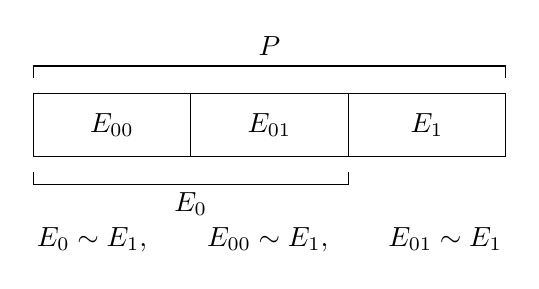
\begin{tikzpicture}[x=1cm,y=1cm]
\draw (0,0) rectangle (6,0.8);
\draw (2,0) -- (2,0.8);
\draw (4,0) -- (4,0.8);
\node at (1,0.4) {$E_{00}$};
\node at (3,0.4) {$E_{01}$};
\node at (5,0.4) {$E_1$};
\draw (0,1) -- (0,1.15) -- (6,1.15) -- (6,1);
\node at (3,1.4) {$P$};
\draw (0,-0.2) -- (0,-0.35) -- (4,-0.35) -- (4,-0.2);
\node at (2,-0.6) {$E_0$};
\node at (3,-1.05) {$E_0\sim E_1,\qquad E_{00}\sim E_1,\qquad E_{01}\sim E_1$};
\end{tikzpicture}
\caption{The decompositions $P=E_0+E_1$ and $E_0=E_{00}+E_{01}$,
shown schematically. The three disjoint cells are orthogonal; the
bracketed corner $E_0$ contains its two children. Here $\sim$ denotes
the equivalence in \eqref{eq:corner-equivalence}.}
\label{fig:kernel-corners}
\end{figure}

Fix $z\in\ker\pi$ and let $z_Q$ denote its image under the
coefficient map $a\mapsto\psi(a)Q$ for each of these idempotents.
Lemma~\ref{lem:corner-comparison}, applied three times with the
second corner $E_1$, gives
\begin{equation}\label{eq:four-corner-equality}
 z_{E_0}=z_{E_1}=z_{E_{00}}=z_{E_{01}}.
\end{equation}
By additivity, the second split in \eqref{eq:four-corner-splits}
splits every root image into its two child images.
Lemma~\ref{lem:orthogonal-root-images} permits their factors to be
collected separately in any word.  Hence
\[
 z_{E_0}=z_{E_{00}}z_{E_{01}}=z_{E_0}^{\,2},
\]
so $z_{E_0}=1$ and then $z_{E_1}=1$.
Finally $\psi(a)P=\psi(a)$.  The first split in
\eqref{eq:four-corner-splits}, with the same commutation argument,
therefore gives
\[
 \theta(z)=z_P=z_{E_0}z_{E_1}=1.
\]
\end{proof}

For $R=B\otimes_k B^{\mathrm{op}}$ and
$\psi=\phi\otimes\phi^{\mathrm{op}}$, the elements $P,U_i,V_i$
constructed in Section~\ref{sec:reduction} satisfy the support and
commutation hypotheses and the pair identities \eqref{eq:ring-pairs}.
Theorem~\ref{thm:kernel} therefore applies to the Steinberg transition
of Section~\ref{sec:affine}: it annihilates the matrix kernel in one step.

\section{The two-transitive envelope}\label{sec:action}

We now turn the algebraic construction into the required permutation
representation.  Proposition~\ref{prop:affine} and
Lemma~\ref{lem:transition} give the finitely presented group
\[
 \Gamma_0=B^6\rtimes\St_6(R)
\]
and its endomorphism $\Theta=(\phi^{(6)},\theta)$.
Theorem~\ref{thm:kernel} says that $\theta$ kills the kernel of the matrix
map.  A mapping torus will remove this kernel while retaining finite
presentation.  We then use the simple subalgebra $A\subseteq B$ to obtain
two-transitivity.

\subsection{The mapping torus and its linear part}

We first record explicitly why a mapping torus has the needed description
even when its defining endomorphism is not injective.

\begin{lemma}\label{lem:mapping-torus}
Let $Q$ be a group and $f:Q\to Q$ an endomorphism.  Write
$L=\varinjlim(Q,f)$, with classes $[q,j]$ for $j\geq0$ and the convention
$[q,j]=[f(q),j+1]$.  The map
\[
 \alpha([q,j])=[q,j+1]
\]
is an automorphism of $L$, and
\[
 \langle Q,t\mid t^{-1}qt=f(q)\ (q\in Q)\rangle
 \cong L\rtimes_\alpha\mathbb Z.
\]
If $Q$ is finitely presented, so is this group.
\end{lemma}

\begin{proof}
Equality in the direct limit means equality after sufficiently many
forward transitions.  Thus $\alpha$ is well defined, as is
$\beta([q,j])=[f(q),j]$.  The defining equivalence gives
$\alpha\beta=\beta\alpha=\mathrm{id}$.
Let $t$ act on $L$ by $\alpha$.  Then
\[
 t^{-1}[q,0]t=\beta([q,0])=[f(q),0],
\]
so the displayed presentation maps to $L\rtimes_\alpha\mathbb Z$.
In the other direction, send
\[
 [q,j]\longmapsto t^jqt^{-j}.
\]
The relation $t^{-1}qt=f(q)$ implies
$t^{j+1}f(q)t^{-(j+1)}=t^jqt^{-j}$, proving that this map is well
defined.  It intertwines $\alpha$ with conjugation by $t$, and hence
extends to a homomorphism from the semidirect product.  The two maps are
inverse on $Q$ and $t$.

For a finite presentation $Q=\langle X\mid\mathcal R\rangle$, choose a
word representing $f(x)$ for each $x\in X$.  Adjoin $t$ and the finitely
many relations $t^{-1}xt=f(x)$ for $x\in X$.  These imply the required
relations for every element of $Q$, since both conjugation and $f$ are
homomorphisms.
\end{proof}

Apply Lemma~\ref{lem:mapping-torus} to $(\Gamma_0,\Theta)$ and denote
the resulting finitely presented group by $\Gamma$.  Put
\[
 M_\infty=\varinjlim((B,+),\phi),\qquad
 E_\infty=\varinjlim(\E_6(R),F),
 \qquad F(g)=I+\psi^{(6)}(g-I).
\]
The transition $F$ is the injective homomorphism of
Lemma~\ref{lem:transition}; recall the matrix map
$\pi:\St_6(R)\to\E_6(R)$.

\begin{lemma}\label{lem:affine-limit}
There are compatible isomorphisms
\[
 \varinjlim(\Gamma_0,\Theta)
 \cong M_\infty^6\rtimes E_\infty,
 \qquad
 \Gamma\cong(M_\infty^6\rtimes E_\infty)\rtimes\mathbb Z.
\]
In the second isomorphism, conjugation by $t$ shifts the stage index
forward by one on both $M_\infty$ and $E_\infty$.
\end{lemma}

\begin{proof}
The square $\pi\theta=F\pi$ induces a surjection from the
Steinberg direct limit to $E_\infty$.  If a class represented by
$h\in\St_6(R)$ maps to the identity, some iterate of $F$ sends
$\pi(h)$ to $I$.  Since $F$ is injective, $\pi(h)=I$ already.
Theorem~\ref{thm:kernel} now gives $\theta(h)=1$, so that class is
trivial.

The compatibility of the module action is
\begin{equation}\label{eq:action-transition}
 \phi^{(6)}(g v)=F(g)\phi^{(6)}(v)
 \qquad(g\in\E_6(R),\ v\in B^6).
\end{equation}
Indeed $\phi(r\cdot b)=\psi(r)\cdot\phi(b)$ for $r\in R$ and
$b\in B$, and separating $g$ into $I+(g-I)$ gives exactly the
modified-identity formula for $F$.  Thus matrices and vectors act on one
another after passage to any common stage.

The stage maps
\[
 (v,h)\longmapsto([v,j],[\pi(h),j])
\]
therefore induce a homomorphism from $\varinjlim(\Gamma_0,\Theta)$ to
$M_\infty^6\rtimes E_\infty$.  It is surjective: choose a common stage
for a vector and a matrix, and then choose a Steinberg preimage of that
matrix.  If a representative $(v,h)$ maps to the identity, injectivity
of $\phi$ gives $v=0$, and injectivity of $F$ gives $\pi(h)=I$.
Consequently $\Theta(v,h)=(0,1)$ by Theorem~\ref{thm:kernel}.  The
homomorphism is injective.  The construction respects stage shifts, so
Lemma~\ref{lem:mapping-torus} gives the second isomorphism as well.
\end{proof}

\subsection{A faithful action and two-transitivity}

Set $X=M_\infty^6$. The subgroup $M_\infty^6$ acts on $X$ by
translations, and $E_\infty$ acts by matrices after passing to a common
stage, as in \eqref{eq:action-transition}. Let $t$ act by the forward
stage shift. This shift intertwines the matrix actions, so these formulas define an
action of $\Gamma$ on $X$.

\begin{proposition}\label{prop:two-transitive-action}
The set $X$ is countably infinite.  The action of $\Gamma$ on $X$ is
faithful and two-transitive, and all its point stabilizers are finitely
generated.
\end{proposition}

\begin{proof}
\emph{The stage filtration.}
Since $\phi$ is injective, identify the $j$th additive stage with its
image $M_j\subseteq M_\infty$, and put $X_j=M_j^6$.  The stages are
nested because $[b,j]=[\phi(b),j+1]$.  They are strictly nested:
every $\phi(b)$ satisfies $p\phi(b)=\phi(b)$, where
$p=\phi(1_B)\ne1_B$, so $1_B$ cannot belong to $\phi(B)$.
Thus $[1_B,j+1]\notin M_j$, and
\begin{equation}\label{eq:strict-stages}
 X_0\subsetneq X_1\subsetneq X_2\subsetneq\cdots.
\end{equation}
The algebra $B$ is countable, being a quotient of the free associative
algebra over the finite field $k$ on finitely many generators.
Consequently $X=\bigcup_{j\geq0}X_j$ is countable; the strict inclusions
make it infinite.

\emph{Faithfulness of the affine part.}
Take a nonidentity element of $E_\infty$, represented by a matrix
$g\ne I$ at stage $j$.  Choose a nonzero entry $r$ of $g-I$, say in
row $a$ and column $b$.  At stage $j+1$, let $v$ have $b_*$ in
coordinate $b$ and zero in the other coordinates.  The $a$th coordinate
of $F(g)v-v$ is
\[
 \psi(r)\cdot b_*\ne0
\]
by Theorem~\ref{thm:algebra-package}.  It remains nonzero in the direct
limit because $\phi$ is injective.  This proves faithfulness of the
linear action.  If an affine element acts identically, evaluating it
at zero first makes its translation zero; linear faithfulness then
makes the element trivial.

\emph{Faithfulness of the whole group.}
Every affine limit element and its inverse have representatives at
some common stage.  At every later stage their translation vectors,
matrices, and inverse matrices act within that stage.  Hence, for each
affine limit element $a$,
\begin{equation}\label{eq:eventual-stage-preservation}
 a(X_j)=X_j\qquad\text{for all sufficiently large }j.
\end{equation}
In contrast,
\[
 t^k(X_j)=X_{j+k}
 \qquad\text{whenever }j\geq0\text{ and }j+k\geq0.
\]
For $k\ne0$, this differs from $X_j$ by
\eqref{eq:strict-stages}.  Thus no nonzero power of $t$ agrees, as a
permutation, with an affine limit element.  If $a t^k$ acts trivially,
then $t^k$ acts as $a^{-1}$, forcing $k=0$ by
\eqref{eq:eventual-stage-preservation}.  Affine faithfulness then gives
$a=1$.

\emph{Two-transitivity.}
We show that $E_\infty$ is transitive on the nonzero vectors of $X$.
Given two such vectors, choose a common representing stage and advance
once more.  All their coordinates now lie in $A$, since
$\phi(B)\subseteq A$, and the vectors remain nonzero.  We work in this
one stage, with the same simple algebra $A$ and its identity $e$.

If a vector has a nonzero coordinate $m_j\in A$, simplicity gives
$A m_j A=A$: the finite sums of elements $a m_j b$ form a nonzero
two-sided ideal.  Thus, for any $d\in A$, there are finitely many
$a_\nu,b_\nu\in A$ with
\[
 d=\sum_\nu a_\nu m_j b_\nu.
\]
The coefficient $r=\sum_\nu a_\nu\otimes b_\nu^{\op}\in R$ then
satisfies $r\cdot m_j=d$.  For $l\ne j$, an elementary matrix in row
$l$, column $j$, with coefficient $r$ adds $d$ to coordinate $l$ and
changes no other coordinate.  It can therefore set that coordinate to
any prescribed value in $A$.

If $j\ne6$, set the last coordinate to $e$.  If $j=6$, first set
coordinate $1$ to $e$, then use it to set the last coordinate to $e$.
Use the last coordinate to kill all the others.  This sends the vector
to $(0,0,0,0,0,e)$.  Applying the procedure to both original vectors
sends them to the same vector at the same stage, proving the asserted
linear transitivity.  Translations, followed by these linear maps and
another translation, take any ordered pair of distinct points to any
other such pair.  The action is two-transitive.

\emph{Point stabilizers.}
Both $E_\infty$ and $t$ fix zero, so the semidirect-product description
gives
\[
 \operatorname{Stab}_\Gamma(0)=E_\infty\rtimes\langle t\rangle
 \cong\Gamma/X.
\]
This is a finitely generated group, since $\Gamma$ is finitely
presented.  More explicitly, $t$ and the images of a finite generating
set of the base Steinberg group generate it: conjugating by positive
powers of $t$ reaches every linear stage.  All other point stabilizers
are conjugate to this one, since translations act transitively.
\end{proof}

\subsection{Embedding the input group and finishing the proof}

The last step is to put the original group into the elementary matrix
part of $\Gamma$.  Here the commutator property of
Lemma~\ref{lem:group-input} is essential.

\begin{proof}[Proof of Theorem~\ref{thm:envelope}]
Let $\widehat G$ be the auxiliary group of
Lemma~\ref{lem:group-input}.  Theorem~\ref{thm:algebra-package} supplies
an injective homomorphism $\iota:\widehat G\to A^\times$, where units
in $A$ have identity $e$.  Define
\[
 \nu(h)=1_B-e+\iota(h)\qquad(h\in\widehat G).
\]
The element $1_B-e$ annihilates $A$ on both sides.  Consequently
\[
 \nu(h)\nu(h')=\nu(hh'),\qquad
 \nu(h)^{-1}=\nu(h^{-1}).
\]
Injectivity of $\iota$ proves injectivity of $\nu$.  Composing with the
injective unital map $B\to R$, $b\mapsto b\otimes1_B$, gives a group
embedding $\bar\nu:\widehat G\to R^\times$.  The tensor map is
injective because $B$ is a nonzero vector space over $k$.

For $u\in R^\times$, let $D_{ij}(u)$ be the diagonal matrix with
entries $u,u^{-1}$ in positions $i,j$ and $1$ elsewhere.  Equation~
\eqref{eq:balanced-diagonal} shows that $D_{ij}(u)\in\E_6(R)$.
Let $s$ be the stable letter in $\widehat G$ and set
\[
 a_g=\bar\nu((g,g)),\qquad b=\bar\nu(s).
\]
By Lemma~\ref{lem:group-input},
$[a_g,b]=\bar\nu((g,1))$.  Taking the commutator of balanced diagonal
matrices on two different pairs of coordinates gives
\[
 [D_{12}(a_g),D_{13}(b)]
 =\operatorname{diag}\bigl(\bar\nu((g,1)),1,1,1,1,1\bigr).
\]
Thus the injective homomorphism given by the diagonal on the right
has image in $\E_6(R)$.  Since the transition $F$ is injective, this
embeds $G$ in $E_\infty$, and hence in $\Gamma$ by
Lemma~\ref{lem:affine-limit}.  Proposition~\ref{prop:two-transitive-action}
and the finite presentation of $\Gamma$ give all the remaining
assertions of Theorem~\ref{thm:envelope}.
\end{proof}

\begin{proof}[Proof of Theorem~\ref{thm:main}]
Suppose first that $G$ is finitely generated and has decidable word
problem.  Theorem~\ref{thm:envelope} embeds it in a finitely presented
group $\Gamma$ with a faithful two-transitive action on a countably
infinite set and finitely generated point stabilizers.  There is exactly one orbit on unordered
two-element subsets.  These are all the hypotheses of
Theorem~\ref{thm:zaremsky}, which embeds $\Gamma$ in a finitely
presented simple group $S$.  The group $S$ is nontrivial, since
$\Gamma$ acts transitively on an infinite set.  This proves the
required direction, including trivial and finite input groups.

For the converse, we give the classical decision argument attributed
by Boone and Higman to Kuznetsov \cite[p.~52]{BH74}.
Let $S=\langle Y\mid\mathcal R\rangle$ be a nontrivial
finitely presented simple group.  On an input word $w$, run the
following two searches in parallel:
\begin{enumerate}[label=(\roman*)]
 \item enumerate presentation proofs that $w=1$ follows from
       $\mathcal R$;
 \item enumerate, for every $y\in Y$, a presentation proof that
       $y=1$ follows from $\mathcal R\cup\{w\}$, stopping when
       a proof has been found for every generator.
\end{enumerate}
Consequences of a finite group presentation are recursively enumerable,
by enumerating finite products of conjugates of relators and their
inverses.  If $w=1$ in $S$, the first search succeeds, whereas the
second cannot succeed for every generator because $S$ is nontrivial.
If $w\ne1$, its normal closure in the simple group $S$ is all of $S$;
thus the second search succeeds for each of the finitely many
generators, whereas the first never succeeds.  Exactly one search
terminates, deciding the word problem in $S$.

For a finitely generated subgroup of $S$, fix words in $Y$ representing
its generators and substitute these words into each input.  This
transfers the decider to that subgroup.  Finally, the same substitution
argument between any two finite generating sets of a group proves
that decidability of its word problem is independent of the chosen
finite generating set.
\end{proof}

\section{The algebra construction}\label{sec:algebra}

We now prove Theorem~\ref{thm:algebra-package}.  The construction has two
parts.  A pair of monoids supplies a simple algebra and an embedding into
a finitely presented algebra.  Partial affine maps then give a corner
with two equivalent orthogonal subcorners.  A separator in the
monoid construction will prove the tensor detection property.

\subsection{The monoid input}

We first define the auxiliary monoid used in the construction.  Let
\(\mathcal P\) be the monoid of partial maps of \(\mathbb Q\) generated by
the full affine maps
\[
 u(x)=x/2,\qquad v(x)=(x+1)/2,
\]
their inverses, and the partial identities \(e_0,e_1\) on
\([0,\infty)\cap\mathbb Q\) and \([1,\infty)\cap\mathbb Q\), respectively.
Composition applies the right-hand factor first.  The identity
\(1_{\mathcal P}\) is the full identity map.

\begin{lemma}\label{lem:partial-affine}
The monoid \(\mathcal P\) has decidable word problem.  Each of its elements
is a map \(x\mapsto ax+b\) on a nonempty rational tail
\([r,\infty)\cap\mathbb Q\), or on all of \(\mathbb Q\), where
\(a=2^m\) for some \(m\in\mathbb Z\), and \(b,r\) are dyadic rationals.
\end{lemma}

\begin{proof}
Represent a full domain by \(r=-\infty\).  The composition of the data
\((a,b,r)\) and \((c,d,s)\) is
\[
 \left(ac,ad+b,\max\{s,(r-d)/c\}\right).
\]
The generators have such data, and the displayed operation preserves
them.  Each domain is infinite, so two represented maps agree precisely
when their domains, slopes and intercepts agree.  The data and their
comparison are computable using dyadic arithmetic.
\end{proof}

For a monoid \(K\) with zero \(\Omega\ne1_K\), write
\[
 T=(K\setminus\{\Omega\})\times\mathcal P\ \sqcup\ \{0_T\}.
\]
The element \(0_T\) is absorbing.  Nonzero pairs multiply
coordinatewise, except that a product whose \(K\)-coordinate is
\(\Omega\) is replaced by \(0_T\).  Its identity is
\((1_K,1_{\mathcal P})\).

\begin{theorem}\label{thm:monoids}
Let \(\widehat G\) be a finitely generated group with decidable word
problem.  There exist a finitely presented monoid \(K\) with zero
\(\Omega\ne1_K\), and a finitely generated monoid \(H\) with decidable
word problem and zero \(\zeta\ne1_H\), with the following properties.
\begin{enumerate}[label=\textup{(\roman*)}]
\item There is an injective group homomorphism
\(\widehat G\longrightarrow H^\times\).
\item For the monoid \(T\) defined above, there is an injective unital
monoid homomorphism \(\kappa:T\longrightarrow H\) with
\(\kappa(0_T)=\zeta\).
\item For every finite ordered tuple \(h_1,\ldots,h_d\) of distinct
nonzero elements of \(H\), with \(d\ge1\), there are \(L,R\in H\)
such that
\[
 Lh_1R=1_H,\qquad Lh_iR=\zeta\quad(2\le i\le d).
\]
\item There is an injective multiplicative map \(c:H\longrightarrow K\)
whose image is disjoint from \(\{1_K,\Omega\}\).  We write
\(c_h=c(h)\); this map is not required to preserve identities or zeros.
\item There is an element \(z\in H\) such that the map
\[
 (\tau,\tau')\longmapsto\kappa(\tau)z\kappa(\tau')
\]
is an injection from \((T\setminus\{0_T\})^2\) into
\(H\setminus\{\zeta\}\).
\end{enumerate}
\end{theorem}

The proof of Theorem~\ref{thm:monoids} occupies
Section~\ref{sec:bootstrap}, using the finite compiler proved in
Appendix~\ref{sec:compiler}. In the construction, \(\zeta\) is the zero
symbol and \(z\) is the class of a distinct separator letter
\(\mathtt z\).

\subsection{A simple algebra inside a finitely presented algebra}

Throughout this section \(k=\mathbb F_2\).
For any monoid \(D\) with zero \(0_D\ne1_D\), its contracted monoid
algebra \(k_0[D]\) has \(k\)-basis \(D\setminus\{0_D\}\).  Basis
elements multiply as in \(D\), with a product equal to \(0_D\)
interpreted as the zero vector.  It is a unital algebra, with identity
the basis element \(1_D\).

To prove Theorem~\ref{thm:algebra-package} for a given group \(L\),
apply Theorem~\ref{thm:monoids} with \(\widehat G=L\) and set
\[
 A_0=k_0[H],\qquad B=k_0[K].
\]
Both algebras are nonzero.  We distinguish the monoid elements
\(\zeta,\Omega\) from algebra zero, and distinguish \(c_{\zeta}\)
from all three: it is a nonzero basis element of \(B\).

The monoid requirements now serve distinct purposes. The selectors
in Theorem~\ref{thm:monoids}(iii) isolate one coefficient of a nonzero
element of \(A_0\), forcing simplicity. The maps in (ii) and (iv)
provide algebra embeddings in opposite directions, but treat zero
differently: \(\kappa\) preserves it, whereas the linear extension
of \(c\) requires a correction by \(c_{\zeta}\). Finally, the
separator in (v) keeps the ordered pairs indexing a tensor basis
distinct, which will supply the tensor detector.

\begin{lemma}\label{lem:algebra-embeddings}
The algebra \(A_0\) is simple, the algebra \(B\) is finitely presented,
and there are injective algebra homomorphisms
\[
 i:A_0\longrightarrow B,
 \qquad
 \rho:B\otimes_k k[\mathcal P]\longrightarrow A_0.
\]
The map \(\rho\) is unital.  The map \(i\) is nonunital and has support identity
\(e=i(1_{A_0})\ne1_B\).
\end{lemma}

\begin{proof}
Let \(a=\sum_{j=1}^d\lambda_jh_j\) be a nonzero element of \(A_0\),
with distinct nonzero support elements \(h_j\) and nonzero coefficients
\(\lambda_j\in k\).  Choose the selectors from
Theorem~\ref{thm:monoids}(iii).  In the contracted algebra they give
\(LaR=\lambda_1 1_{A_0}\).  Hence every nonzero two-sided ideal contains
the identity, proving simplicity.  This argument also covers a support
element equal to \(1_H\).

The linear extension of \(c\) alone would not respect the contraction
of the zero class, since \(c_{\zeta}\ne\Omega\). For \(h\ne\zeta\), define
\[
 i(h)=c_h-c_{\zeta}
\]
and extend linearly.  Multiplicativity of \(c\) gives
\[
 c_hc_{h'}=c_{hh'},\qquad
 c_hc_{\zeta}=c_{\zeta}c_h=c_{\zeta},\qquad
 c_{\zeta}^2=c_{\zeta}.
\]
Consequently
\[
 (c_h-c_{\zeta})(c_{h'}-c_{\zeta})=c_{hh'}-c_{\zeta}.
\]
When \(hh'=\zeta\), this is zero, as required.  The vectors \(c_h\)
are distinct nonzero basis elements of \(B\).  In particular, the
coefficient of \(c_h\), for \(h\ne\zeta\), in \(i(a)\) is exactly
the coefficient of \(h\) in \(a\), proving injectivity.  Its support
identity is
\[
 e=c_{1_H}-c_{\zeta},\qquad e^2=e,
 \qquad ei(a)=i(a)e=i(a).
\]
Neither basis vector in this expression is \(1_K\); therefore
\(e\ne1_B\), and indeed \(1_B\notin i(A_0)\).

A finite presentation for \(B\) is obtained from the finite monoid
presentation for \(K\).  We may adjoin a generator \(\Omega\) and a
relation identifying it with a word representing the zero, so that
\(\Omega\) is a presentation letter.  Take the same generators in a free associative
unital \(k\)-algebra, replace every equation \(u=v\) by \(u-v=0\),
and impose \(\Omega=0\).  To verify this presentation, first omit the
last relation.  The ideal of binomial relations is precisely the span
of all differences of words in the same monoid congruence class.
One inclusion follows because each contextual use of a defining
equation belongs to the ideal, and a chain of such uses telescopes.
The reverse inclusion follows by mapping each word to its congruence
class in the free vector space on \(K\).  The quotient thus has basis
\(K\); imposing \(\Omega=0\) removes exactly its absorbing zero
class.  It gives \(B\).  Adding the relation \(2\cdot1=0\) to the same
generators and relations also presents \(B\) as a unital ring.

Finally, nonzero basis pairs give a unital algebra isomorphism
\[
 B\otimes_k k[\mathcal P]\cong k_0[T].
\]
It sends \(b\otimes p\), for basis elements \(b\ne\Omega\) and
\(p\in\mathcal P\), to \((b,p)\); products that acquire
\(K\)-coordinate \(\Omega\) vanish on both sides. The linear extension
of \(\kappa\) gives the required injective unital map \(\rho\).
\end{proof}

Identify \(A=i(A_0)\subseteq B\).  It is a simple algebra with its own
identity \(e\), and Theorem~\ref{thm:monoids}(i) embeds
\(L\) in \(A^\times\): a unit of \(H\) and its inverse
give inverse basis elements in \(A_0\), which \(i\) sends to units
relative to \(e\).  We next construct an injective nonunital
endomorphism of \(B\) whose image lies in \(A\).

\subsection{Two equivalent subcorners}

For a dyadic rational \(a\), let \(e_a\) denote the partial identity
on \([a,\infty)\cap\mathbb Q\).  These maps belong to \(\mathcal P\):
\(u^{-1}v\) is translation by \(1\), its powers and conjugates by
powers of \(u\) give all dyadic translations, and conjugating \(e_0\)
by translation by \(a\) gives \(e_a\).  In the monoid itself,
\begin{equation}\label{eq:tail-identities}
 e_a e_b=e_{\max\{a,b\}},\qquad
 w e_a w^{-1}=e_{w(a)}
\end{equation}
for every available full increasing affine map \(w\).  Thus these
are equalities of basis elements in the abstract algebra
\(k[\mathcal P]\).

We require a nonzero corner that decomposes into two orthogonal copies
of itself. The identities in the next lemma have the rectangular-inverse
form familiar from Leavitt's module-type construction
\cite[Section~3]{Leavitt1962}, with the corner idempotent as identity.
Here we realize them directly using the partial affine maps above.

\begin{lemma}\label{lem:binary-tail-corner}
There is a nonzero idempotent \(q\in k[\mathcal P]\) and elements
\(s'_0,s'_1,t'_0,t'_1\in qk[\mathcal P]q\) such that
\[
 t'_i s'_j=\delta_{ij}q,\qquad
 s'_0t'_0+s'_1t'_1=q.
\]
\end{lemma}

\begin{proof}
Set \(q=e_0-e_1\).  Its two basis elements and \(1_{\mathcal P}\)
are distinct, so \(q\ne0,1\);
Equation~\eqref{eq:tail-identities} gives \(q^2=q\).  Put
\[
 w_0=u,\quad w_1=v,\qquad
 q_0=w_0qw_0^{-1}=e_0-e_{1/2},\quad
 q_1=w_1qw_1^{-1}=e_{1/2}-e_1.
\]
Using the same tail identities and expanding in the monoid basis gives
\[
 q_0^2=q_0,\quad q_1^2=q_1,\quad q_0+q_1=q,
 \quad q_0q_1=q_1q_0=0.
\]
For example,
\(q_0q_1=e_{1/2}-e_1-e_{1/2}+e_1=0\).
In particular \(qq_j=q_jq=q_j\).

Define \(s'_j=w_jq\) and \(t'_j=qw_j^{-1}\).  Then
\(s'_jt'_j=q_j\) and \(t'_js'_j=q\).  The identities
\(s'_j=q_jw_j\) and \(t'_j=w_j^{-1}q_j\), together with
\(qq_j=q_jq=q_j\), show
\[
 qs'_j=s'_jq=s'_j,\qquad qt'_j=t'_jq=t'_j.
\]
Moreover \(t'_jq_j=t'_j\) and \(q_js'_j=s'_j\).  For \(i\ne j\)
we therefore have
\[
 t'_is'_j=t'_iq_iq_js'_j=0.
\]
Finally \(\sum_j s'_jt'_j=q_0+q_1=q\).  All calculations use
Equation~\eqref{eq:tail-identities} and linear operations in
\(k[\mathcal P]\).
\end{proof}

Define
\[
 j:B\longrightarrow A_0,\qquad j(b)=\rho(b\otimes q),
 \qquad \phi=i\circ j:B\longrightarrow B.
\]
These maps are nonunital algebra homomorphisms.  The map \(j\) is multiplicative because \(q^2=q\), and it is injective
because \(q\ne0\) and tensor products are over the field \(k\).
Hence \(\phi\) is injective and \(\phi(B)\subseteq A\).  Let
\[
 p=\phi(1_B),\qquad
 s_l=i\rho(1_B\otimes s'_l),\qquad
 t_l=i\rho(1_B\otimes t'_l)\quad(l=0,1).
\]
The idempotent \(p\) belongs to \(A\), so \(p\ne1_B\).
Applying the two algebra maps to Lemma~\ref{lem:binary-tail-corner}
gives
\begin{equation}\label{eq:B-corner-pairs}
 s_l,t_l\in pBp,\qquad
 t_ls_j=\delta_{lj}p,\qquad s_0t_0+s_1t_1=p.
\end{equation}
These elements commute with \(\phi(B)\).  Indeed,
\[
 (b\otimes q)(1_B\otimes s'_l)=b\otimes s'_l
   =(1_B\otimes s'_l)(b\otimes q),
\]
and the identical calculation holds for \(t'_l\); now apply
\(i\rho\). Thus the required self-embedding and binary pairs
centralizing \(\phi(B)\) have been constructed. It remains to verify detection
for the tensor action.

\subsection{A separating tensor vector}

As in Section~\ref{sec:affine}, set \(R=B\otimes_k B^{\mathrm{op}}\),
acting on \(B\) by \((a\otimes b^{\mathrm{op}})m=amb\), and define
\[
 \psi=\phi\otimes\phi^{\mathrm{op}}.
\]
We need one vector on which \(\psi(r)\) acts nontrivially for every
\(r\ne0\). The separator gives this simultaneously for all
\(r\), by realizing distinct basis tensors as distinct monoid elements.

Let \(W=\rho(B\otimes_k k[\mathcal P])\subseteq A_0\), with basis
\(\{\kappa(\tau):\tau\in T\setminus\{0_T\}\}\).  Part (v) of
Theorem~\ref{thm:monoids} proves that the linear map
\[
 D:W\otimes_k W^{\mathrm{op}}\longrightarrow A_0,
 \qquad D(x\otimes y^{\mathrm{op}})=xzy,
\]
is injective: it sends distinct basis tensors to distinct nonzero basis
elements of \(A_0\).  This includes tensors with an identity factor.
Since \(j(B)\subseteq W\), the composite
\[
 R\xrightarrow{\ j\otimes j^{\mathrm{op}}\ }
 W\otimes_k W^{\mathrm{op}}
 \xrightarrow{\ D\ } A_0
 \xrightarrow{\ i\ } B
\]
is a sequence of injective linear maps.  For
\(r=\sum_{\nu}a_{\nu}\otimes b_{\nu}^{\mathrm{op}}\),
its value is
\[
 \begin{aligned}
 i\bigl(D((j\otimes j^{\mathrm{op}})(r))\bigr)
   &=\sum_{\nu}i(j(a_{\nu}))\,i(z)\,i(j(b_{\nu}))\\
   &=\psi(r)\cdot i(z).
 \end{aligned}
\]
Thus \(b_*=i(z)\) satisfies
\begin{equation}\label{eq:tensor-detection}
 r\ne0\quad\Longrightarrow\quad\psi(r)\cdot b_*\ne0.
\end{equation}
The assertion concerns the action after \(\psi\); its proof uses the
explicit separator vector.

\begin{proof}[Proof of Theorem~\ref{thm:algebra-package}]
The algebra \(B\) is nonzero and finitely presented by
Lemma~\ref{lem:algebra-embeddings}.  Its subalgebra \(A=i(A_0)\) is
simple with identity \(e\), and contains \(L\) in its unit
group.  The map \(\phi\) is injective, has image in \(A\), and has
proper support \(p\).  Equation~\eqref{eq:B-corner-pairs} supplies
the binary pairs centralizing \(\phi(B)\), which give the tensor identities
\eqref{eq:ring-pairs} as explained in Section~\ref{sec:reduction}. Finally,
Equation~\eqref{eq:tensor-detection} supplies the required vector
\(b_*\).  These are all the asserted data.
\end{proof}

\section{Coding with a decreasing dependency bound}
\label{sec:bootstrap}

We prove Theorem~\ref{thm:monoids}.  The two monoids in that theorem
must contain information about one another: the finitely presented monoid
will multiply representatives of the decidable monoid, while the latter
will contain a coded copy of the former.  We arrange this using a program
whose evaluations on words of length $n$ depend only on its values at
strictly smaller lengths.  The other ingredient is a family of separated
words that supplies the finite-tuple selectors.

\subsection{The bounded compiler}

Fix a finite alphabet $\Sigma$ containing the disjoint triples
\[
 (\mathtt b_T,\mathtt a_T,\mathtt c_T),\qquad
 (\mathtt b_G,\mathtt a_G,\mathtt c_G)
\]
and the six further letters
$\mathtt z,\mathtt d,\mathtt l,\mathtt r,\mathtt h,\zeta$.
Fix a total order with $\mathtt a_T<\mathtt c_T$ and
$\mathtt a_G<\mathtt c_G$.  Words are ordered by \emph{shortlex}:
first by length and then lexicographically.  We use an acceptable
programming system for partial functions $\Sigma^*\to\Sigma^*$, writing
$f_\eta$ for the function with index $\eta$.  In particular, universal
evaluation and effective substitution of parameters are available;
integers and tuples are represented by fixed computable word encodings.

The following finite construction is proved in
Appendix~\ref{sec:compiler}.  Its conditional statement is essential:
the program index determines the presentation without running the
program. The evaluator is also fixed independently of a length bound;
its termination and compatibility with equations will be proved from
the program's behavior within that bound.

\begin{lemma}[Bounded compiler]\label{lem:compiler}
From a program index $\eta$ one can compute a finite monoid presentation
$K_\eta$ with a zero letter $\Omega$, a finite presentation alphabet
$X_\eta$, and an additive grade $\gamma$ on words, such that
$0\le\gamma(x)\le M=2$ for every letter and $\gamma(\Omega)=0$.
There is a partial word algorithm $N_\eta$, independent of any budget,
with the following properties.

The alphabet contains letters $\alpha,\mathsf Q,\omega$ and right
anchor letters $a_R$ for $a\in\Sigma$, all mutually distinct and
different from $\Omega$. For a word $u$, let $u_R$ replace each
letter $a$ by $a_R$, and set
\[
 \operatorname{raw}(u)=\alpha\mathsf Q u_R\omega\qquad(u\in\Sigma^*).
\]
Unconditionally, the algorithm fixes the empty word, $\Omega$, and
every literal word $\operatorname{raw}(u)$, and sends every word
containing $\Omega$ to $\Omega$. On an input word $a$, its only calls
to $f_\eta$ are on words of length at most $\gamma(a)$; apart from
those calls it performs finite computations.

Suppose that, for some integer $m\ge0$,
\begin{align}
 &f_\eta(w)\text{ is defined and }|f_\eta(w)|\le |w|
       &&(|w|\le m),\label{eq:budget-total}\\
 &f_\eta(xf_\eta(w)y)=f_\eta(xwy)
       &&(|xwy|\le m).\label{eq:budget-context}
\end{align}
Then $N_\eta$ terminates on all words of grade at most $m$.
Each such word is joined to its literal output by a finite derivation
in the presentation whose intermediate grades do not exceed the input
grade.  A single presentation equation, used in any context, preserves
the output whenever both endpoints have grade at most $m$.
Consequently
\begin{equation}\label{eq:bounded-context}
 N_\eta(u)=N_\eta(v)\quad\Longrightarrow\quad
 N_\eta(xuy)=N_\eta(xvy)
 \quad\text{if }\gamma(xuy),\gamma(xvy)\le m.
\end{equation}

If
\eqref{eq:budget-total}--\eqref{eq:budget-context} hold for all $m$,
then $N_\eta$ decides equality in $K_\eta$ and
\begin{equation}\label{eq:raw-product}
 N_\eta\bigl(\operatorname{raw}(u)\operatorname{raw}(v)\bigr)=\operatorname{raw}\bigl(f_\eta(uv)\bigr).
\end{equation}
The presentation is computed without evaluating $f_\eta$.
\end{lemma}

For clarity, \eqref{eq:bounded-context} follows from the preceding
derivation statement.  Transplant the paths from $u$ and $v$ to their
common output into $x(-)y$.  Neither contextual path leaves the budget,
so one-step invariance identifies their outputs.  A general machine
encoding without this bounded conclusion would not suffice below.
The raw singleton rule has a different role: it will distinguish the
elements used for the injection $H\to K$. Multiplication of two raw
words, rather than evaluation of a singleton, will encode the product
in $H$ through \eqref{eq:raw-product}.

\subsection{Codes and finite rule tables}

First consider any index $\eta$.  The auxiliary monoid $\mathcal P$
has decidable equality by Lemma~\ref{lem:partial-affine}.

Let $Y$ be the disjoint union of $X_\eta$ and a fixed finite generating
alphabet for $\mathcal P$.  For a $Y$-word $v$, write $v_K,v_{\mathcal P}$
for its projections, obtained by deleting the letters of the other
alphabet.  Its \emph{tested class} is zero if $N_\eta(v_K)=\Omega$;
otherwise it is the pair consisting of $N_\eta(v_K)$ and the value of
$v_{\mathcal P}$ in $\mathcal P$.  This is at present a partial test.
For the second type of code, fix a finite monoid generating alphabet
$Z$ for $\widehat G$, including the inverses of a finite group
generating set, and test words by their values in $\widehat G$.
This second test is total by the hypothesis of Theorem~\ref{thm:monoids}.

Choose computably an integer $D_0>M$ such that
$2^{D_0-1}\ge\max\{|Y|,|Z|\}$.  Encode the letters of $Y$, in their
chosen order, by distinct words beginning with $\mathtt b_T$ and
followed by $D_0-1$ letters from
$\{\mathtt a_T,\mathtt c_T\}$, in lexicographic order.  Encode $Z$
in the same way using the other triple.  Write $C(v)$ for concatenation
of the appropriate codes and put $C(\varepsilon)=\varepsilon$.
The type of a nonempty code sequence is unambiguous.  Codes preserve
shortlex comparison and have length $D_0$ per generator.

Enumerate all nonempty finite ordered tuples
\[
 (w_1^{(j)},\ldots,w_{s_j}^{(j)})\qquad(j\ge1)
\]
of distinct $\Sigma$-words avoiding $\zeta$; the empty word is allowed
as a member.  Choose integers $N_j$ recursively so that
\begin{equation}\label{eq:envelope-spacing}
 N_j>j,\qquad N_j>\max_i|w_i^{(j)}|,\qquad
 N_j>2N_h+2+\max_i|w_i^{(h)}|\quad(h<j).
\end{equation}
These inequalities concern \emph{all potential} earlier envelopes,
regardless of which rules will be selected.  The increasing sequence
$N_j$ is computable without performing any tested-class evaluation.

We now define a partial procedure $F(\eta,w)$.  Put $n=|w|$ and form
the following finite rule table $\mathcal R_n$.
\begin{enumerate}
\item Include $\zeta a\to\zeta$ and $a\zeta\to\zeta$ for every
letter $a\in\Sigma$.  For each nonempty $Y$-word $v$ with
$D_0|v|\le n$, test its class.  If it is zero, include
$C(v)\to\zeta$.  Otherwise find the shortlex least word $v'$ of the
same tested class among all words of length at most $|v|$, including
the empty word; include $C(v)\to C(v')$ if $v'\ne v$.
Do the same for $Z$-words using equality in $\widehat G$, with no
zero case.  Call these the \emph{static rules}.

\item Process the tuples with $N_j\le n$ in order.  If every member
of tuple $j$ has no reducible occurrence under the static rules and
previously selected rules, include
\begin{equation}\label{eq:selector-rules}
 \mathtt d\mathtt l^{N_j}w_i^{(j)}\mathtt r^{N_j}\mathtt h
 \longrightarrow
 \begin{cases}
 \varepsilon,&i=1,\\
 \zeta,&i>1.
 \end{cases}
\end{equation}
Some of these left sides may be longer than $n$; they simply cannot
act on the input.

\item Reduce $w$ until no rule applies, using a fixed deterministic
choice of occurrence and rule.
\end{enumerate}
Whenever the tests terminate, the last step terminates: every rule
decreases shortlex.  In particular a nonempty code reduced to $\zeta$
shortens, since $D_0>2$.  All other non-code rules shorten as well.
Thus $F$ is uniformly partial computable.

\subsection{The fixed point and its length induction}

Effective substitution of parameters gives a total computable index
transformation $\tau(\eta)$ for the function $F(\eta,-)$.  Kleene's
Recursion Theorem~\cite{Kleene38} supplies an index with
\begin{equation}\label{eq:fixed-point}
 f_\eta(w)=F(\eta,w)
\end{equation}
as partial functions.  Here is the short parameterization argument.
Let $U$ be universal evaluation and let $d(a)$ be an effectively
obtained index for the partial function
$w\mapsto U(U(a,a),w)$.  Choose an index $b$ computing the total
function $a\mapsto\tau(d(a))$.  For $\eta=d(b)$,
\[
 U(\eta,w)=U(U(b,b),w)=U(\tau(d(b)),w)=F(\eta,w).
\]
Only now fix the presentation alphabet and code length belonging to
this particular $\eta$.  There is no advance bound on the machine's
size or working space.  Write $f=f_\eta$ and $K=K_\eta$.

\begin{lemma}\label{lem:bootstrap}
The function $f$ is total and length-nonincreasing.  The rule tables
are stable on bounded-length words: for $k\le n$, $\mathcal R_k$
and $\mathcal R_n$ have the same rules whose left sides have length
at most $k$.  Each $\mathcal R_n$ is confluent on words of length at
most $n$, and
\begin{equation}\label{eq:f-context}
 f(xf(w)y)=f(xwy)\qquad(x,w,y\in\Sigma^*).
\end{equation}
\end{lemma}

\begin{proof}
We prove all bounded assertions together by induction on $n$.
For $n=0$, there are no tested classes or tuple decisions, and the
empty word is unchanged.  Suppose $n>0$ and the assertions are known
at smaller bounds.  Every use of $N_\eta$ in a static test, including
each candidate in a least-representative search, uses a $Y$-word of length at most
$\lfloor n/D_0\rfloor$.  Its $K$-projection has grade at most
\begin{equation}\label{eq:strict-dependency}
 m=M\lfloor n/D_0\rfloor<n.
\end{equation}
The induction hypothesis supplies
\eqref{eq:budget-total}--\eqref{eq:budget-context} at $m$.
Lemma~\ref{lem:compiler} therefore makes all these tests terminate.
There are only finitely many tests and tuple decisions, and the
subsequent shortlex-decreasing reduction terminates.

We first establish stability.  For a fixed generator word $v$, its
static rule is determined by the same tests and the same candidates
of length at most $|v|$ at every larger bound.  Consider a tuple with
$N_j\le k\le n$.  Each tested body has length less than $N_j$, hence
less than $k$.  New static left sides longer than $k$ cannot occur
in it.  Induction over earlier tuple numbers shows that the previously
selected rules that can occur in the bodies also agree.  Hence the
decision for tuple $j$ agrees at both bounds.  A new tuple with
$N_j>k$ has every selector side longer than $k$, so cannot add a rule
on a word of length at most $k$.  This proves stability, including
the decisions for selected rules too long to act at the smaller bound.

It remains to prove local confluence for $\mathcal R_n$.  All
reductions stay inside the length-at-most-$n$ ball.  Disjoint
occurrences can be reduced in either order. If the word contains
$\zeta$, every branch still contains it: absorption retains $\zeta$,
and no other rule has a left side containing that letter. Absorption joins all
branches at $\zeta$.  We check the other overlaps explicitly.

\smallskip\noindent
\emph{Selectors from different stages.}
Let the older left side have total length $L$, and let the newer one
be $\mathtt d\mathtt l^N w\mathtt r^N\mathtt h$.
By \eqref{eq:envelope-spacing}, $L<N$ and $|w|<N$.
A nonempty old suffix cannot equal a new prefix: the former ends in
$\mathtt h$, while a prefix of length at most $L$ lies in the initial
$\mathtt d\mathtt l^N$.  An old prefix cannot equal a new suffix,
since their first letters are respectively $\mathtt d$ and either
$\mathtt r$ or $\mathtt h$.  These exclude both orientations of a
proper boundary overlap.  For containment, an old occurrence cannot
start at the new initial $\mathtt d$, because its terminal
$\mathtt h$ would lie in the initial $\mathtt l$-run.  Any other
start must be in the body.  It cannot leave the body: it cannot end
in the final $\mathtt r$-run, and reaching the final $\mathtt h$
would require crossing a run longer than the entire old side.
Thus it would lie wholly in the body, contrary to the newer tuple's
irreducibility test.

\smallskip\noindent
\emph{Selectors from one stage.}
A second start strictly inside one side must lie in its body.
There are then fewer than $N$ body letters left before the final
$\mathtt r$-run, so that start cannot be followed by $N$ consecutive
$\mathtt l$'s.  If two sides start at the same place and their body
lengths differ, the terminal $\mathtt h$ of the shorter falls in the
final $\mathtt r$-run of the longer, because both body lengths are
less than $N$.  Equal body lengths force equal bodies, hence the same
rule, as tuple members are distinct.  This also covers an empty body.

\smallskip\noindent
\emph{A code and a selector.}
Code letters are disjoint from the envelope markers.  An overlapping
code side would therefore have to lie wholly inside the selector's
body.  The static irreducibility test excluded this.  All static sides
short enough to occur there were already present when the tuple was
processed, because the body's length is less than $N_j$.

\smallskip\noindent
\emph{Two code sides.}
They have the same type and aligned starts: within a code sequence,
$\mathtt b_T$ or $\mathtt b_G$ occurs only at a block boundary.
Their union is therefore an entire code sequence $C(v)$, of length
at most $n$.  For group codes, a replacement preserves the value of
this union by group multiplication.  For product codes, replacing
a subword by a nonzero tested-equal word preserves the tested class
of the union by \eqref{eq:bounded-context} and equality in
$\mathcal P$.  Indeed each old or new union has generator length
at most $\lfloor n/D_0\rfloor$, and hence its $K$-projection has
grade at most $m$.  We use this bound separately for both endpoints:
a shorter generator word need not have smaller actual $K$-grade.

If a subword tests zero, apply \eqref{eq:bounded-context} to its
$K$-projection and $\Omega$, whose grade is zero.  The contextual
word containing $\Omega$ has output $\Omega$, so the union also
tests zero.  Hence if one branch introduces $\zeta$, it reduces the
whole union to $\zeta$, and the other either does the same or retains
a zero-class code sequence, to which its whole-word zero rule applies.
That remaining sequence cannot be empty, since
$N_\eta(\varepsilon)=\varepsilon\ne\Omega$.
The same argument covers a zero-class union when both first
replacements are code sequences.

If the union class is nonzero, let $v_*$ be its least representative
among words of length at most $|v|$.  Either branch yields a word
$v_b$ of the same class with $|v_b|\le|v|$.  Since $v_b$ is one of
the candidates defining $v_*$, we have
$|v_*|\le|v_b|$, and $v_*$ is also the least candidate within this
smaller bound.  Each branch therefore reduces by its whole-word rule
to $C(v_*)$, unless it already equals that word.  The representative
$v_*$ may be empty; no empty left side is needed.  These joining
reductions can be made on the union before acting on any newly
adjacent outside letters.

This exhausts the local peaks.  Termination and local confluence give
confluence on the ball by Newman's Lemma~\cite{Newman42}.
Indeed, by well-founded induction, assume every proper descendant of
a word has a unique normal form.  Any two first steps have a common
descendant by local confluence; the induction hypothesis makes their
normal forms equal, proving uniqueness for the original word and
hence confluence.  Finally, if $|xwy|\le n$,
perform inside $x(-)y$ the normalization of $w$ computed at bound
$|w|$.  By stability every rule used belongs to $\mathcal R_n$, and
length never increases.  Confluence gives
$f(xf(w)y)=f(xwy)$.  This establishes the budget hypotheses at $n$
and completes the induction.
\end{proof}

\subsection{The two monoids and their embeddings}

Let $H$ be the monoid on $\Sigma$ whose equations are the union of
all the rule tables.  Every word is related to its computed normal
form, which is irreducible for this union by stability.
Conversely, a contextual use of any one
equation preserves that form: choose a bound containing both
endpoints and the equation, and apply stability and confluence from
Lemma~\ref{lem:bootstrap}.  Thus two words represent the same element
of $H$ if and only if their literal $f$-outputs agree.  This proves
decidability.  The empty word and the single letter $\zeta$ are
distinct irreducibles; they represent the identity and the absorbing
zero of $H$.

The budget hypotheses now hold at every length, so
Lemma~\ref{lem:compiler} gives an equality test for $K$.  In
particular its identity and zero are distinct.  The tested product
classes are now the actual elements of
\[
 T=\bigl((K\setminus\{\Omega\})\times\mathcal P\bigr)\cup\{0_T\},
\]
with coordinatewise multiplication and every pair having first
coordinate $\Omega$ collapsed to zero.
Here a letter of $X_\eta$ acts in the first coordinate and a
generator of $\mathcal P$ in the second; the letter $\Omega$ maps to
$0_T$.  Thus $Y$ generates $T$.

For a nonzero element of $T$, take its least shortlex $Y$-representative
$v$.  The code $C(v)$ is irreducible: a subcode rule would either
force the element to be zero or produce a smaller representative;
no selector or absorption side occurs in a pure code word.
Every other representative reduces by its whole-word rule to this
same code, and every zero-class code reduces to $\zeta$.
Consequently coding defines an injective zero-preserving monoid map
\[
 \kappa:T\longrightarrow H.
\]
It is unital because the least representative of the identity is
empty, and it is multiplicative because codes concatenate.
The identical argument for $Z$-words embeds $\widehat G$ unitally in
$H$.  Its image consists of units, since the products of mutually
inverse group words have the empty representative.  This includes
the trivial group and does not require a nonempty generating set.

Let $z\in H$ be represented by the separator $\mathtt z$.
For least representatives $v,v'$ of nonzero elements of $T$, the words
\begin{equation}\label{eq:separator-words}
 C(v)\mathtt z C(v')
\end{equation}
are irreducible.  No code crosses the separator; each code portion
is already irreducible; and there are no selector markers or
$\zeta$.  These literal words recover the ordered pair, including
when one or both representatives are empty.  They are nonzero
because none equals $\zeta$.  This proves the separator assertion
of Theorem~\ref{thm:monoids}.

\subsection{Selectors and multiplication by raw words}

Take any ordered tuple of distinct nonzero elements
$h_1,\ldots,h_s$ of $H$, and let $w_1,\ldots,w_s$ be their normal
words.  These words avoid $\zeta$, since any word containing it
reduces to the zero word.  Their tuple occurs in the enumeration,
say at stage $j$.  A word irreducible for the final rule set is
irreducible for the static and selected rules present at stage $j$.
Hence this tuple passes its test.  With
\[
 L=\mathtt d\mathtt l^{N_j},\qquad
 R=\mathtt r^{N_j}\mathtt h
\]
as elements of $H$, the selected equations give
$Lh_1R=1$ and $Lh_iR=\zeta$ for $i>1$.  The argument includes a tuple
containing the identity, whose normal representative is empty.

Finally define a multiplicative map in the opposite direction by
\[
 c:H\longrightarrow K,\qquad c([w])=[\operatorname{raw}(f(w))].
\]
The normal-form characterization of $H$ makes this well-defined.
Every raw singleton is its own literal $N_\eta$-output.  Distinct
normal words therefore give distinct elements of $K$, and none of
these elements is its identity or its zero.  For normal words $u,v$,
\eqref{eq:raw-product} gives
\[
 c([u])c([v])=[\operatorname{raw}(f(uv))]=c([uv]).
\]
Thus $c$ is injective and multiplicative, as required.  It is not
unital: even $c(1)=[\operatorname{raw}(\varepsilon)]$ is distinct from $1_K$.
Also $c(\zeta)\ne\Omega$; it is absorbing only within $c(H)$.
The finite presentation of $K$ came from the compiler, while the
finite alphabet and normal-form procedure give the claimed finite
generation and decidability of $H$.  All conclusions of
Theorem~\ref{thm:monoids} are proved.

\appendix
\section{The finite compiler}\label{sec:compiler}

We prove Lemma~\ref{lem:compiler}. The input is a program index $\eta$
for a partial function $f_\eta:\Sigma^*\rightharpoonup\Sigma^*$ on the
fixed finite alphabet $\Sigma$. We construct a finite monoid presentation
and its partial evaluator. The main issue is to control arbitrary words
in that presentation, including malformed machine configurations.

Encoding a finite machine by contextual equations, and checking the
consequences of using those equations in reverse, are classical ideas
\cite[pp.~3--6]{Post1947}.
Murskii used finite machine presentations to embed finitely generated
recursively presented semigroups in finitely presented semigroups
\cite[Theorem~1.2 and Section~1.5]{Murskii1967}; his construction also
controls malformed initial configurations \cite[Section~2.4]{Murskii1967}.
For the present construction we also need a single evaluator on all
presentation words, normalization paths that never increase grade,
and invariance under equations in arbitrary contexts within the grade
bound. We prove these properties explicitly below.

Fix a deterministic one-tape machine for $f_\eta$, with tape cells indexed
by the nonnegative integers. A left move at cell zero stays there. The
input begins at cell zero and is followed by blanks; a returned string
also begins at zero and ends at its first blank. We use an effective
compilation of the acceptable programming system into this convention.
The resulting finite transition table is part of the compiler's input;
constructing the presentation never runs the program.

\subsection{Cells, paths, and the validator}

A \emph{cell} consists of an immutable base in
$\Sigma\sqcup\{\mathsf C,\mathsf D,\mathsf W\}$ and a finite tag.
Bases in $\Sigma$ are called anchors. The other bases mark two cuts and
a workspace cell. A tag has an anchor-read bit, a workspace-filled bit,
a work symbol from the compiled machine's finite tape alphabet, an
output-reading bit, and an output mark in $\Sigma\sqcup\{\mathrm{none}\}$.
The \emph{clean} tag has every bit unset, work symbol blank, and output
mark none. All these fields may be included on every base; fields not
used there are simply left unchanged. A bare cell base in a rule means
the cell with its entire tag clean.

The presentation has a zero letter $\Omega$ and the arrows of the quiver
in Figure~\ref{fig:compiler-quiver}. There are arrows
$\alpha:O\to L$ and $\omega:R\to O$, head arrows $L\to R$, and two
loop copies $b_L,b_R$ of every tagged cell $b$, at $L,R$, respectively.
There are no vertex-identity generators: the empty word is the global
identity. Add the equations making $\Omega$ absorbing and making every
incompatible pair of arrows equal to $\Omega$.

\begin{figure}[ht]
\centering
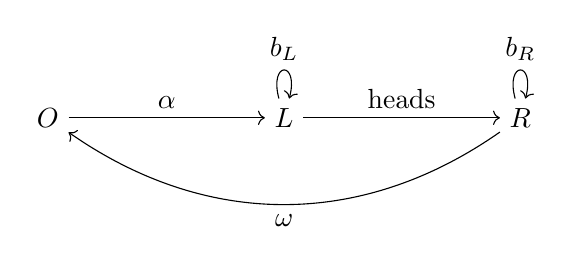
\begin{tikzpicture}[scale=1]
\node (O) at (0,0) {$O$};
\node (L) at (3,0) {$L$};
\node (R) at (6,0) {$R$};
\draw[->] (O) -- node[above] {$\alpha$} (L);
\draw[->] (L) -- node[above] {heads} (R);
\draw[->] (R) to[bend left=35] node[below] {$\omega$} (O);
\draw[->] (L) to[loop above] node[above] {$b_L$} (L);
\draw[->] (R) to[loop above] node[above] {$b_R$} (R);
\end{tikzpicture}
\caption{Nonzero words are paths. Cutting at each interior visit
$\omega\alpha$ to $O$ leaves sectors with at most one head.}
\label{fig:compiler-quiver}
\end{figure}

A nonempty path is cut at every $\omega\alpha$ into \emph{sectors}.
Each contains at most one head, since returning from $R$ to $L$
requires such a cut. A headed sector has optional $\alpha$, left loops,
a head, right loops, and optional $\omega$. Sectors without heads
are allowed. Thus the same notation describes complete computations
and words with missing boundaries.

Assign grade zero to $\Omega$ and workspace cells, grade two to cut cells
with base $\mathsf C$, and grade one to all other generators. Tags do
not affect grade. Extend grade additively to words, writing $\gamma$.
The maximum generator grade is therefore $M=2$. Workspace can be added
without increasing grade, although it increases literal word length.

Use raw and quota heads $\mathsf Q,\mathsf P$, validator heads
$\mathsf I,\mathsf J,\mathsf J',\mathsf N,\mathsf V$, a disjoint set of
machine heads, and a cleanup head $\mathsf Z$.
For an anchor word $x$, the notation $x_L$ or $x_R$ means its sequence
of clean cell copies. A sector is \emph{full raw} if it has the form
\[
\operatorname{raw}(x)=\alpha\mathsf Q x_R\omega,
\qquad x\in\Sigma^*.
\]
The word $x$ is its payload. To combine two such sectors, first impose
\begin{align}
\mathsf Q a_R&=a_L\mathsf Q &&(a\in\Sigma),\label{eq:compiler-slide}\\
\mathsf Q\omega\alpha\mathsf Q&=\mathsf C_L\mathsf P\mathsf D_R,
&\mathsf P\mathsf D_R&=\mathsf W_L\mathsf P\mathsf D_R,
&\mathsf P\mathsf D_R&=\mathsf I\mathsf D_R.
\label{eq:compiler-entry}
\end{align}
In the following validator equations, the arrows specify the forward
direction used to analyze the machine; the defining relations are
equations in both directions:
\begin{align}
\mathsf W_L\mathsf I&\longrightarrow\mathsf I\mathsf W_R,
&\mathsf C_L\mathsf I&\longrightarrow\mathsf J\mathsf C_R,
&a_L\mathsf J&\longrightarrow\mathsf J a_R,\nonumber\\
\alpha\mathsf J&\longrightarrow\alpha\mathsf J',
&\mathsf J'a_R&\longrightarrow a_L\mathsf J',
&\mathsf J'\mathsf C_R&\longrightarrow\mathsf C_L\mathsf N,
\label{eq:compiler-validation}\\
\mathsf N\mathsf W_R&\longrightarrow\mathsf W_L\mathsf N,
&\mathsf N\mathsf D_R&\longrightarrow\mathsf D_L\mathsf V,
&\mathsf V a_R&\longrightarrow a_L\mathsf V,
&\mathsf V\omega&\longrightarrow q_{\rm start}\omega.\nonumber
\end{align}
The anchor rules range over $a\in\Sigma$.

An \emph{entry} has head $\mathsf I$ immediately before clean
$\mathsf D_R$. The validator reaches $q_{\rm start}$ from an entry
only when that entry has the complete form
\begin{equation}\label{eq:compiler-clean-entry}
\alpha x_L\mathsf C_L\mathsf W_L^s\mathsf I\mathsf D_R y_R\omega,
\qquad x,y\in\Sigma^*,\quad s\geq0.
\end{equation}
Indeed the first left sweep checks precisely the clean workspace up to
$\mathsf C$, and the next checks only clean anchors up to $\alpha$.
The rightward sweeps then check these anchors, the first cut, the
workspace, the second cut, and only clean anchors up to $\omega$.
Thus both boundaries and every tag are checked. At the handoff all cells
are on the left of the head.

These relations prepare a raw product for computation. Slide the first
head across $x$, merge the two adjacent heads, insert $s$ workspace
cells, and enter the validator. The simulation and cleanup defined
below will complete the following passage whenever $f_\eta(xy)$ is
defined and has length at most $|xy|$, provided $s$ is sufficiently large:
\begin{equation}\label{eq:compiler-pipeline}
\begin{aligned}
\operatorname{raw}(x)\operatorname{raw}(y)
&\ \rightsquigarrow\ 
\alpha x_L\mathsf C_L\mathsf W_L^s\mathsf I\mathsf D_R y_R\omega\\
&\ \rightsquigarrow\ 
\operatorname{raw}\bigl(f_\eta(xy)\bigr).
\end{aligned}
\end{equation}
The first passage is the preparation just described; the second is
validation, simulation on the workspace, and cleanup. The two anchor
blocks retain the input $xy$ and provide space for its output letters.

Successful computations alone do not control the presented monoid,
because each equation can also be used in reverse. The validator and
simulator will preserve the ordered cell bases and have finitely many
tags and head states. Consequently their transitions on any fixed
sector form a finite graph, even if the simulated program never halts.
We will search its whole weak component---allowing transitions in
either direction---to normalize arbitrary configurations. The component
analysis will distinguish those that contain an entry from those that
do not. Quota insertion is kept outside this finite graph.

\subsection{A finite transition table for the computation}

We specify the remaining machine equations explicitly through finite
scan instructions. This makes the construction uniform in $\eta$ while
avoiding a separate list of rules for each tape symbol.

Every state has one designated reading side. A right-reading state has,
for each tested tagged cell, at most one rule of either form
\begin{equation}\label{eq:compiler-instructions}
q b_R\longrightarrow b'_Lq'
\quad\hbox{or}\quad
q b_R\longrightarrow q'b'_R;
\end{equation}
a left-reading state uses the mirrored forms. These instructions cross
the cell or stay in the same gap, respectively. The cells $b,b'$ always
have the same base. Boundary tests are stationary rules
$\alpha q\to\alpha q'$ or $q\omega\to q'\omega$ on the designated
side. A failed test has no rule. A finite cell predicate expands into
the list of tagged cells satisfying it; complementary cases are
disjoint. Finite registers are incorporated into the state set by a
finite Cartesian product.

Here are the scan instructions used below, together with their complete
expansion convention.
\begin{itemize}
\item To rewind, cross every cell on the left unchanged. At $\alpha$,
  change state without moving and start the specified right-reading
  continuation. If $\alpha$ is absent, the scan gets stuck at the left
  end of the word.
\item To find the first cell satisfying a predicate, test cells on the
  right. At a failure cross unchanged and repeat. At a match use the
  specified stationary update and continuation. At $\omega$, use the
  specified end continuation, or get stuck if failure was prescribed.
\item To go to the right boundary, cross all right cells unchanged and
  use the specified stationary continuation at $\omega$.
\end{itemize}
All invocations are expanded with distinct phase states, apart from
explicit repetitions of a loop. In particular $q_{\rm start}$ is fresh:
its only incoming rule is the validator handoff, and its only outgoing
rule is $q_{\rm start}\omega\to q_{\rm rewind}\omega$, where
$q_{\rm rewind}$ starts the first rewind. No continuation returns to
$q_{\rm start}$ or to a validator state.

The following finite control program supplies all further internal
machine equations.
\begin{enumerate}
\item \emph{Copy the input.} Rewind, and find the first anchor whose read
  bit is unset. Set that bit, carry its base $a$ in finite state, rewind,
  and find the first workspace cell whose filled bit is unset. Write
  $a$ on its work track and set its filled bit. Failure to find that
  workspace cell is stuck. Rewind and repeat the anchor search.

  When the anchor search reaches $\omega$, rewind and check that an
  unfilled workspace cell remains; otherwise get stuck. Rewind once
  more and locate the first workspace cell for simulation. On
  \eqref{eq:compiler-clean-entry} this writes exactly $xy$ in anchor
  order into the initial workspace cells, followed by a blank.

\item \emph{Run the given machine.} The simulated head reads a workspace
  cell on its right. For each machine state and work symbol, expand its
  single transition using \eqref{eq:compiler-instructions}. A stationary
  move writes and stays. A right move writes and crosses the current
  cell, and the next simulation state requires another workspace cell
  on the right. A left move first writes without crossing, then enters
  a left-reading intermediate state. That state crosses an immediately
  left workspace cell unchanged, or stays if the immediately left base
  is $\mathsf C$; any other case is stuck. It then returns to a
  right-reading simulation state. This implements the left-end
  convention. A halt is recognized only at a workspace cell in bounds.

\item \emph{Read the output.} After halt, rewind and find the first
  workspace cell whose output-reading bit is unset. A blank work symbol
  ends the output. For a work symbol $a\in\Sigma$, set that bit, carry
  $a$ in finite state, rewind, and place output mark $a$ on the first
  anchor whose output mark is none. Failure to find such an anchor is
  stuck. Rewind and repeat. An invalid output symbol, or exhaustion of
  the workspace without a blank, is stuck. When output ends, go to
  $\omega$ and enter a fresh state $q_{\rm ok}$, with no outgoing
  internal transition.
\end{enumerate}

Each instruction uses only the finite predicates, finite registers, and
updates just specified. Expanding all cases gives a finite list of
equations computable from the machine table. Each state tests only its
designated side and has disjoint cases. Consequently the internal
forward transition relation has outdegree at most one on \emph{every}
sector, including sectors with missing boundaries and arbitrary tags.
Every transition preserves the number and ordered bases of the cells.

On a passing entry, simulation success computes $f_\eta(xy)$ genuinely.
Conversely, if $f_\eta(xy)$ is defined and has length at most $|xy|$,
then some finite quota $s$ permits success: take more workspace cells
than the input length, the largest tape index visited by the halting
computation, and the output length. The extra cell supplies its blank
delimiter. There are $|xy|$ anchors for the output marks. This includes
empty input: at least one workspace cell is supplied, and a length bound
forces the output to be empty.

Add the exit equation $q_{\rm ok}\omega\to\mathsf Z\omega$ and the
following cleanup equations. An anchor cell $b$ with output mark
$a\in\Sigma$ has
\begin{equation}\label{eq:compiler-cleanup}
b_L\mathsf Z\longrightarrow\mathsf Z a_R.
\end{equation}
For every other tagged cell use $b_L\mathsf Z\to\mathsf Z$, and add
$\alpha\mathsf Z\to\alpha\mathsf Q$. Cleanup is deterministic and
never increases grade, even on dirty data. Applied to a successful
passing entry, it leaves
\begin{equation}\label{eq:compiler-success}
\alpha\mathsf Q f_\eta(xy)_R\omega.
\end{equation}
The leftward sweep places successive output letters on its right in the
correct order. All unused anchors and all nonanchor cells disappear.

\subsection{Finite components on arbitrary sectors}

We now analyze sectors with arbitrary tags and optional boundaries.
For a validator or machine sector, form the graph of internal forward
transitions, excluding entry from $\mathsf P$ and exit to $\mathsf Z$.
We use its entire weak connected component. The ordered bases of its
cells and its boundary flags are fixed. If there are $k$ cells and $h$
internal head states, with at most $c$ tags per cell, there are at most
$(k+1)h c^k$ possible configurations with these data. Its weak component
can therefore be found by a finite search through elementary compiled
steps. This search does not call $f_\eta$ or wait for a computation to
halt. In particular, the quota insertion rule is excluded: finite grade
alone would not bound the number of grade-zero workspace cells.

\begin{lemma}\label{lem:compiler-components}
Every internal weak component has at most one entry and at most one
sector whose head is $q_{\rm ok}$ immediately before its final $\omega$.
If both occur, the forward computation from the entry reaches that
sector and has the clean form and genuine output
described in \eqref{eq:compiler-clean-entry} and
\eqref{eq:compiler-success}.
\end{lemma}
\begin{proof}
An entry has internal indegree zero: the only possible predecessor of an
$\mathsf I$-sector is a left sweep, whose output has clean $\mathsf W$
immediately right of the head, whereas an entry has clean $\mathsf D$.
Every other validator sector has indegree at most one. For head
$\mathsf J$, its possible predecessor types are distinguished by clean
$\mathsf C$ versus an anchor immediately right. For $\mathsf J'$ they
are distinguished by $\alpha$ versus an anchor immediately left; for
$\mathsf N$ by clean $\mathsf C$ versus $\mathsf W$ immediately left;
and for $\mathsf V$ by clean $\mathsf D$ versus an anchor immediately
left. There are no transitions from machine states to validator states.

The validator phases progress in their displayed order, and each sweep
is finite. An entry whose validation fails before handoff therefore
belongs to an isolated finite chain: its vertices have at most one
predecessor and one successor, the entry has no predecessor, and the
failed end has no successor. It shares its component with no other
entry. Every passing entry has
\eqref{eq:compiler-clean-entry}. Its fixed base sequence and boundary
flags determine it uniquely, including its clean tags and the head gap
immediately before the unique $\mathsf D$. Hence there is at most one
entry in any component.

Finally, a finite directed graph with outdegree at most one has a single
eventual cycle or terminal vertex in each weak component. Indeed the
unique forward trajectories of adjacent vertices have the same eventual
object, and this propagates along weak paths. A sector ending in
$q_{\rm ok}\omega$ is terminal. Thus it is the only such sector in its
component, and every forward trajectory there reaches it. If an entry
is present, it therefore passes validation and genuinely succeeds.
\end{proof}

\subsection{The partial evaluator}

The component lemma leaves a choice when both an entry and a successful
terminal occur. Returning to the entry, removing its quota, and undoing
the merge, then sliding the raw heads left, gives
$\operatorname{raw}(x)\operatorname{raw}(y)$;
cleaning up the terminal gives
$\operatorname{raw}(f_\eta(xy))$. We give the entry priority, so that
internal equations have identical preprocessing outputs. The final
combination of consecutive raw sectors will identify the two routes
in \eqref{eq:compiler-pipeline}, using the contextual identity assumed
in Lemma~\ref{lem:compiler} when other raw sectors are adjacent.

This priority also applies to a failed or malformed entry; in that case
quota removal need not produce two full raw sectors. Conversely, a
successful component without an entry need not encode a genuine input
computation. It can use its unique terminal cleanup directly. The
following algorithm includes all these cases.

The algorithm $N_\eta$ preserves the empty word. It sends every word
containing $\Omega$, and every nonpath, to $\Omega$, using the zero
relations. For a nonempty path, first preprocess its sectors as follows.
\begin{enumerate}
\item Leave sectors without heads unchanged. Move $\mathsf Q$ to its
  leftmost reachable gap using \eqref{eq:compiler-slide}, across clean
  anchors only.
\item If $\mathsf P$ has clean $\mathsf D_R$ immediately right, remove
  all immediately preceding clean $\mathsf W_L$ by the quota equation.
  If clean $\mathsf C_L$ is then immediately left, unmerge
  $\mathsf C_L\mathsf P\mathsf D_R$ into
  $\mathsf Q\omega\alpha\mathsf Q$ and normalize the two resulting
  raw heads as above. Otherwise keep the trimmed sector. A
  $\mathsf P$ without immediately right clean $\mathsf D_R$ is kept.
\item Run $\mathsf Z$ cleanup until it is stuck or becomes
  $\mathsf Q$; in the latter case normalize that raw head.
\item For any validator or machine head, find its finite internal weak
  component. If there is an entry, move to it along a weak path, revert
  to $\mathsf P$, and use the preceding rule. If there is no entry but
  there is a sector ending in $q_{\rm ok}\omega$, move there and use
  cleanup. If neither
  exists, use the least sector in the component in shortlex order.
\end{enumerate}
Lemma~\ref{lem:compiler-components} makes the choices in the last rule
unambiguous. The ordering is fixed independently of any grade budget.
All these operations preserve the original outer boundaries; only
unmerge creates an interior $\omega\alpha$ and splits a sector.

Replace each maximal run of $t\geq2$ consecutive full raw sectors,
with payloads $u_1,\ldots,u_t$, by
\begin{equation}\label{eq:compiler-run}
\alpha\mathsf Q f_\eta(u_1\cdots u_t)_R\omega.
\end{equation}
A run of length one is left unchanged, without evaluating $f_\eta$.
This completes the definition of $N_\eta$. Its only calls to that
function are in \eqref{eq:compiler-run}.

Assume now the budget hypothesis of Lemma~\ref{lem:compiler} at $m$.
Every preprocessing operation has a derivation that never raises grade.
Internal component paths preserve every base and hence grade. Raw slides
and entry reversal preserve grade. Quota cells have grade zero. Unmerge
preserves grade because
\[
\gamma(\mathsf C_L\mathsf P\mathsf D_R)=2+1+1
=1+1+1+1=\gamma(\mathsf Q\omega\alpha\mathsf Q).
\]
Cleanup preserves or decreases it. Each argument in
\eqref{eq:compiler-run} has length at most the original total grade,
since every anchor contributes one. Thus all required calls terminate
for an input of grade at most $m$.

The replacement of two full raw sectors is also derivable without
raising grade. Move the first head right across its anchors, merge at
$\mathsf Q\omega\alpha\mathsf Q$, insert a sufficient grade-zero
workspace quota, enter, simulate successfully, and clean up. The result
is the raw word for $f_\eta(u_1u_2)$. Repeating this operation gives
\eqref{eq:compiler-run}, because the budget hypothesis implies
\[
f_\eta\bigl(f_\eta(u_1u_2)u_3\bigr)
=f_\eta(u_1u_2u_3)
\]
and the analogous identities for longer runs. The successive arguments
to $f_\eta$ have length at most $|u_1|+\cdots+|u_t|$, because
$f_\eta$ is length-nonincreasing. Each elementary derivation step
preserves or decreases grade, including the insertion of grade-zero
workspace. Thus every call and every intermediate word remains within
its required budget. This proves termination and the asserted
grade-nonincreasing normalization path.

\subsection{Invariance under equations and contexts}

We verify that one contextual equation step preserves $N_\eta$ when
both endpoints have grade at most $m$. All nonzero equation sides are
nonempty paths with the same initial and terminal vertices. This
includes the deletion $b_L\mathsf Z\to\mathsf Z$. A replacement
therefore preserves whether the whole word is a path. Zero equations
and nonpaths give $\Omega$ on both sides, so it remains to compare paths,
using their sectors in the whole contextualized word.

Raw slides have the same leftmost reachable gap. Quota changes have the
same trimmed sector. Entry from $\mathsf P$ has the same preprocessing
on both sides, since the internal component gives priority to its entry,
even if that entry is malformed and validation fails. Internal
validator or machine equations leave the weak component unchanged.
Cleanup equations give the same result by forward determinism, including
the last step to $\mathsf Q$. A merge is immediately undone by quota
preprocessing before normalizing its two raw heads. This remains true
when the two sectors have incomplete outer boundaries or dirty cells.
In each case the preprocessed sector list is identical, so its subsequent
raw-run replacements agree.

The only remaining equation is
$q_{\rm ok}\omega\to\mathsf Z\omega$. If its internal component has
no entry, both sides use the same unique terminal cleanup. If it has an
entry, Lemma~\ref{lem:compiler-components} says that the entry is
\eqref{eq:compiler-clean-entry} and its computation returns
$f_\eta(xy)$. Entry-priority preprocessing on one side gives two full
raw sectors for $x,y$; cleanup on the other gives a single full raw
sector for $f_\eta(xy)$. With no full raw neighbors, the pair is replaced
by exactly that singleton. Otherwise let $a,b$ be the concatenations of
the neighboring raw words on the left and right. The final runs have
outputs
\[
f_\eta(axyb)
\quad\hbox{and}\quad
f_\eta\bigl(a f_\eta(xy)b\bigr),
\]
which agree by the budget hypothesis. The anchor count $|axyb|$ on the
entry side is at most the original grade, so this use is legitimate.
Passing validation forces both $\alpha$ and $\omega$; an incomplete
sector cannot occur in this exceptional comparison. This proves
equation-step invariance in every context.

If $N_\eta(u)=N_\eta(v)$ and both $xuy,xvy$ have grade at most $m$,
transplant the nonincreasing normalization paths of $u$ and $v$ into
$x(-)y$. Additivity keeps every intermediate word within budget.
Equation-step invariance identifies each input's answer with the answer
of its contextualized normal form. Those two middle strings are
literally equal, proving bounded context compatibility. This argument
does not require sector boundaries to survive the attachment of context.

If the hypotheses hold at every budget, every finite derivation is
covered by some budget. Invariance then implies that equal monoid words
have equal $N_\eta$ answers. The converse follows from each word's
derivation to its answer. Thus $N_\eta$ is an exact word-problem
evaluator. Its definition always leaves each raw singleton
$\alpha\mathsf Q u_R\omega$ literal, distinct from $\Omega$ and from
the empty word; on two such sectors it gives the raw encoding of
$f_\eta(uv)$ whenever the relevant budget hypothesis holds. All parts
of Lemma~\ref{lem:compiler} follow.

\begingroup
\small
\raggedright
\setlength{\bibsep}{4pt}
\bibliographystyle{plainnat}
\bibliography{references}
\endgroup
\end{document}
